\documentclass[conference]{IEEEtran}
\IEEEoverridecommandlockouts
\usepackage{cite}
\usepackage{amsmath,amssymb,amsfonts}
\usepackage{algorithmic}
\usepackage{algorithm}
\usepackage{graphicx}
\usepackage{textcomp}
\usepackage{xcolor}
\usepackage{booktabs}
\usepackage[utf8]{inputenc}
\usepackage[portuguese]{babel}

\def\BibTeX{{\rm B\kern-.05em{\sc i\kern-.025em b}\kern-.08em
    T\kern-.1667em\lower.7ex\hbox{E}\kern-.125emX}}

\begin{document}

\title{Avaliação Experimental Comparativa de Algoritmos Exatos (Branch-and-Bound) e Aproximativos para o Set Covering Problem\\
\thanks{Relatório de Trabalho Prático 2 de DCC207 -- Algoritmos 2, UFMG.}
}

\author{\IEEEauthorblockN{Natanael dos Santos Júnior}
\IEEEauthorblockA{\textit{Departamento de Ciência da Computação} \\
\textit{Universidade Federal de Minas Gerais (UFMG)}\\
Belo Horizonte, Brasil \\
natanaeljunior@dcc.ufmg.br}
}

\maketitle

\begin{abstract}
Este trabalho apresenta uma avaliação experimental comparativa entre um algoritmo aproximativo (heurística Gulosa) e um algoritmo exato (Branch-and-Bound) para o problema de cobertura de conjuntos (Set Covering Problem -- SCP). A implementação do Branch-and-Bound explora diferentes estratégias de busca (DFS e Best-First) associadas a limitantes inferiores baseados em Sum-Degree e Packing. Os algoritmos foram submetidos a testes com bases sintéticas uniformes, adversariais e instâncias de grande escala adaptadas da OR-Library. Os resultados experimentais confirmam que o algoritmo aproximativo possui tempo de processamento sub-segundo de excelente utilidade prática para instâncias grandes, enquanto o Branch-and-Bound é severamente limitado pela dimensão e densidade das instâncias, com o DFS Sum-Degree sobressaindo-se no limiar de transição de fase devido ao menor overhead computacional por nó.
\end{abstract}

\begin{IEEEkeywords}
Set Covering, Branch-and-Bound, Heurística Gulosa, Análise Experimental, Limitantes Inferiores, NP-difícil.
\end{IEEEkeywords}

\section{Introdução}
O problema de cobertura de conjuntos (Set Covering Problem -- SCP) é um clássico problema NP-difícil na ciência da computação e na pesquisa operacional com ampla gama de aplicações práticas, incluindo roteamento de veículos, localização de facilidades e agendamento de tripulação. O problema é formulado sobre um universo de elementos e uma coleção de conjuntos cujos elementos pertencem ao universo, associados a respectivos custos. O objetivo é selecionar um subconjunto de coleções com custo total minimizado de forma que todos os elementos do universo sejam cobertos.

Dada a natureza NP-difícil do SCP, algoritmos exatos tradicionais sofrem com tempo de processamento exponencial, tornando-se proibitivos à medida que a escala do problema cresce. Para contornar esse gargalo, heurísticas aproximativas rápidas (como a heurística Gulosa) são adotadas na prática comercial para encontrar soluções de boa qualidade em tempo polinomial.

Este trabalho prático tem como objetivo principal avaliar o desempenho computacional (tempo de execução, uso de memória e qualidade da solução) de ambas as abordagens. Apresentamos a análise empírica comparando a heurística Gulosa contra diferentes configurações de Branch-and-Bound sobre instâncias sintéticas controladas e instâncias reais representativas do repositório padronizado OR-Library (Beasley).

\section{Trabalhos Relacionados}
Devido ao seu amplo escopo de aplicação prática e complexidade teórica intrínseca, o Set Covering Problem (SCP) tem sido extensivamente estudado nas últimas décadas. As abordagens propostas na literatura dividem-se principalmente em métodos exatos, heurísticas clássicas e metaheurísticas.

Os métodos exatos visam provar a otimalidade global da solução. Dentre eles, destacam-se os algoritmos baseados em Programação Linear Inteira (ILP) e técnicas de Branch-and-Bound. Beasley~\cite{b1} propôs algoritmos exatos pioneiros baseados em subgradientes e relaxação Lagrangiana, obtendo limitantes inferiores bastante apertados por meio da resolução do problema dual Lagrangiano. A relaxação Lagrangiana foca em relaxar as restrições difíceis do SCP, penalizando sua violação na função objetivo, o que permite resolver instâncias de médio a grande porte quando combinada com heurísticas de primalização. Mais recentemente, Bläsius et al.~\cite{b2} investigaram a eficiência de limitantes inferiores em Branch-and-Bound modernos, comparando abordagens de empacotamento disjunto (\textit{packing}) e graus de cobertura de conjuntos em problemas de set covering esparsos.

Para problemas de grande escala, onde métodos exatos tornam-se proibitivos devido ao crescimento exponencial do espaço de busca, heurísticas e metaheurísticas são amplamente preferidas. O algoritmo aproximativo clássico baseado em escolhas gulosas (Chvatal~\cite{b3}) é amplamente utilizado por sua simplicidade e garantia teórica de fator de aproximação logarítmico. Por outro lado, metaheurísticas como GRASP (Greedy Randomized Adaptive Search Procedure)~\cite{b4}, Simulated Annealing~\cite{b5} e algoritmos genéticos têm sido aplicados com sucesso para encontrar soluções quase ideais de forma computacionalmente eficiente. Esses métodos combinam a construção gulosa aleatorizada com busca local iterativa, permitindo escapar de ótimos locais.

\section{Métodos e Algoritmos}
O Set Covering Problem (SCP) pode ser formalizado matematicamente como um problema de Programação Linear Inteira (ILP). Dado um universo de elementos $U = \{1, 2, \dots, m\}$ e uma coleção de subconjuntos $\mathcal{S} = \{S_1, S_2, \dots, S_n\}$, onde cada conjunto $S_j \subseteq U$ possui um custo associado $c_j > 0$, o objetivo é encontrar uma subcoleção de custo total mínimo que cubra todos os elementos de $U$.

Definimos a matriz de incidência elemento-conjunto $A \in \{0,1\}^{m \times n}$, cujos elementos $a_{ij}$ são dados por:
\begin{equation}
a_{ij} = \begin{cases} 
1, & \text{se } i \in S_j \\
0, & \text{caso contrário}
\end{cases}
\end{equation}

Seja $x_j \in \{0, 1\}$ a variável de decisão binária que indica se o conjunto $S_j$ foi selecionado ($x_j = 1$) ou não ($x_j = 0$). O modelo de programação linear inteira correspondente é formulado como:
\begin{equation}
\text{Minimizar } \sum_{j=1}^n c_j x_j
\end{equation}
sujeito a:
\begin{equation}
\sum_{j=1}^n a_{ij} x_j \ge 1, \quad \forall i \in \{1, \dots, m\}
\end{equation}
\begin{equation}
x_j \in \{0, 1\}, \quad \forall j \in \{1, \dots, n\}
\end{equation}

A restrição (3) garante que cada elemento $i$ do universo seja coberto por pelo menos um dos conjuntos selecionados, enquanto a restrição (4) impõe a binariedade das decisões.

\subsection{Algoritmo Aproximativo Guloso}
O algoritmo aproximativo seleciona incrementalmente os conjuntos com base em sua eficiência instantânea. A eficiência de um conjunto $S_j$ de custo $c_j$ na iteração $t$ é definida pela razão:
\begin{equation}
\text{Eficiência}(S_j) = \frac{|S_j \cap U_{\text{uncovered}}|}{c_j}
\end{equation}
O algoritmo seleciona repetidamente o conjunto de maior eficiência, remove seus elementos do conjunto de elementos não cobertos $U_{\text{uncovered}}$ e para quando $U_{\text{uncovered}} = \emptyset$. A complexidade assintótica de tempo desta abordagem é $O(\text{iterações} \times n) = O(m \cdot n)$, sendo altamente eficiente na prática. Teoricamente, possui um fator de aproximação garantido de $H(m) = \sum_{i=1}^m 1/i \approx \ln(m) + 1$ em relação ao custo ótimo exato. O fluxo lógico da heurística gulosa é detalhado no Algoritmo~\ref{alg:greedy}.

\begin{algorithm}
\caption{Heurística Gulosa para o SCP}
\label{alg:greedy}
\begin{algorithmic}[1]
\REQUIRE Universo $U$, Coleção de subconjuntos $\mathcal{S}$, Custos $c$
\ENSURE Conjunto de índices selecionados $J$
\STATE $J \leftarrow \emptyset$
\STATE $U_{\text{uncovered}} \leftarrow U$
\WHILE{$U_{\text{uncovered}} \neq \emptyset$}
    \STATE $j^* \leftarrow \operatorname{argmax}_{j \notin J} \frac{|S_j \cap U_{\text{uncovered}}|}{c_j}$
    \STATE $J \leftarrow J \cup \{j^*\}$
    \STATE $U_{\text{uncovered}} \leftarrow U_{\text{uncovered}} \setminus S_{j^*}$
\ENDWHILE
\RETURN $J$
\end{algorithmic}
\end{algorithm}

\subsection{Algoritmo Exato Branch-and-Bound}
O algoritmo Branch-and-Bound (B\&B) resolve o SCP de forma exata navegando em uma árvore binária de decisão (onde cada nó representa a decisão de incluir ou excluir um conjunto). O algoritmo utiliza heurísticas de poda baseadas na comparação do custo acumulado somado a um limitante inferior (\textit{lower bound}) com a melhor solução viável (limite superior) encontrada pelo algoritmo Guloso. O fluxo geral da busca em profundidade (DFS) com poda por limitante inferior está especificado no Algoritmo~\ref{alg:bb}.

\begin{algorithm}
\caption{Algoritmo Branch-and-Bound (DFS)}
\label{alg:bb}
\begin{algorithmic}[1]
\REQUIRE Universo não coberto $U_{\text{uncovered}}$, Conjuntos disponíveis $A_{\text{available}}$, Solução corrente $J_{\text{current}}$, Custo corrente $C_{\text{current}}$
\ENSURE Atualiza melhor custo global $C_{\text{best}}$ e melhor solução $J_{\text{best}}$

\STATE $lb \leftarrow \text{CalcularLimitante}(U_{\text{uncovered}}, A_{\text{available}})$
\IF{$C_{\text{current}} + lb \ge C_{\text{best}}$}
    \STATE \textbf{retornar} \COMMENT{Poda por Limitante Inferior}
\ENDIF
\IF{$U_{\text{uncovered}} == \emptyset$}
    \IF{$C_{\text{current}} < C_{\text{best}}$}
        \STATE $C_{\text{best}} \leftarrow C_{\text{current}}$
        \STATE $J_{\text{best}} \leftarrow J_{\text{current}}$
    \ENDIF
    \STATE \textbf{retornar} \COMMENT{Nova melhor solução viável encontrada}
\ENDIF
\IF{$A_{\text{available}} == \emptyset$}
    \STATE \textbf{retornar} \COMMENT{Inviabilidade do subproblema}
\ENDIF

\STATE Selecionar elemento alvo $e^* \in U_{\text{uncovered}}$ com menor número de conjuntos de cobertura disponíveis
\STATE Obter $S_{\text{covering}} \leftarrow \{ j \in A_{\text{available}} \mid e^* \in S_j \}$
\STATE Ordenar $S_{\text{covering}}$ por eficiência decrescente em relação a $U_{\text{uncovered}}$

\STATE $A_{\text{temp}} \leftarrow A_{\text{available}}$
\FORALL{$S_{j^*} \in S_{\text{covering}}$}
    \STATE $A_{\text{temp}} \leftarrow A_{\text{temp}} \setminus \{j^*\}$
    \STATE $U_{\text{new}} \leftarrow U_{\text{uncovered}} \setminus S_{j^*}$
    \STATE Chamada recursiva: \texttt{BranchAndBound}($U_{\text{new}}, A_{\text{temp}}, J_{\text{current}} \cup \{j^*\}, C_{\text{current}} + c_{j^*}$)
\ENDFOR
\end{algorithmic}
\end{algorithm}

\subsubsection{Estratégias de Busca}
\begin{itemize}
\item \textbf{DFS (Depth-First Search)}: Explora ramos profundos de forma recursiva. Possui custo de memória irrisório ($O(\text{profundidade})$), o que impede estouros de memória em árvores grandes.
\item \textbf{Best-First Search}: Mantém uma fila de prioridades ordenada de forma crescente pelo limitante inferior estimado. Explora primeiro caminhos teoricamente mais promissores. Para evitar explosão de memória RAM (comum em Python devido ao gerenciamento do heap), implementamos uma trava física limitando a fila a no máximo 50.000 nós.
\end{itemize}

\subsubsection{Limitantes Inferiores (Lower Bounds)}
A eficiência das podas no Branch-and-Bound depende fortemente da qualidade dos limitantes inferiores. Adotamos as formulações de Bläsius et al.~\cite{b2}:
\begin{itemize}
\item \textbf{Sum-Degree (Efficiency)}: Este limitante estima o custo mínimo necessário para cobrir os elementos ainda não cobertos com base no grau ativo dos conjuntos disponíveis. Para cada elemento não coberto $e \in U_{\text{uncovered}}$, a contribuição de custo é dada pela menor eficiência dos conjuntos que o cobrem. Formalmente, o limitante $L_{\text{eff}}$ é computado como:
\begin{equation}
L_{\text{eff}} = \sum_{e \in U_{\text{uncovered}}} \min_{S_j \in \text{Cover}(e)} \frac{c_j}{\text{degree}(S_j)}
\end{equation}
onde $\text{Cover}(e) = \{ S_j \in A_{\text{available}} \mid e \in S_j \}$ representa os conjuntos disponíveis que cobrem $e$, e a função $\text{degree}(S_j) = |S_j \cap U_{\text{uncovered}}|$ é a quantidade de elementos não cobertos que $S_j$ pode cobrir no subproblema atual. Caso todos os custos de conjuntos sejam unitários (unicost, $c_j = 1.0$), aplicamos o teto inteiro:
\begin{equation}
L_{\text{eff}} = \left\lceil \sum_{e \in U_{\text{uncovered}}} \min_{S_j \in \text{Cover}(e)} \frac{1}{|S_j \cap U_{\text{uncovered}}|} \right\rceil
\end{equation}
Esse limitante tem complexidade linear de cálculo $O(m \cdot n)$, sendo computacionalmente muito barato, embora menos apertado.

\item \textbf{Packing (Disjoint-Subset)}: Este limitante baseia-se na identificação de um conjunto de elementos não cobertos mutuamente disjuntos, isto é, que não compartilham nenhum conjunto de cobertura disponível em comum. Se dois elementos $e_a, e_b \in U_{\text{uncovered}}$ não podem ser cobertos pelo mesmo conjunto disponível, qualquer solução viável para o subproblema deve selecionar pelo menos dois conjuntos distintos para cobri-los.
Formalmente, buscamos uma coleção de elementos $E_{\text{pack}} \subseteq U_{\text{uncovered}}$ tal que:
\begin{equation}
\forall e_a, e_b \in E_{\text{pack}} \, (a \neq b), \quad \text{Cover}(e_a) \cap \text{Cover}(e_b) = \emptyset
\end{equation}
Sob essa condição, a soma dos custos mínimos necessários para cobrir cada elemento individual em $E_{\text{pack}}$ é um limitante inferior válido:
\begin{equation}
L_{\text{pack}} = \sum_{e \in E_{\text{pack}}} \min_{S_j \in \text{Cover}(e)} c_j
\end{equation}
A busca pelo maior $E_{\text{pack}}$ equivale ao problema de Conjunto Independente Máximo sobre o grafo de conflito dos elementos, que é NP-difícil. Para viabilizar seu cálculo rápido por nó, implementamos uma heurística gulosa: ordenamos os elementos de $U_{\text{uncovered}}$ pelo número de conjuntos que os cobrem (ordem crescente de dificuldade) e selecionamos elementos para $E_{\text{pack}}$ desde que os seus conjuntos de cobertura não se sobreponham aos dos elementos já selecionados. Embora mais apertado, o Packing apresenta complexidade computacional mais elevada.

\item \textbf{Combined (Both)}: A fim de aproveitar o baixo custo de computação do Sum-Degree e o forte poder de poda do Packing, nossa abordagem combinada executa primeiro o cálculo de $L_{\text{eff}}$. Caso o valor obtido somado ao custo corrente já seja suficiente para podar o nó ($C_{\text{current}} + L_{\text{eff}} \ge C_{\text{best}}$), o nó é podado imediatamente e evita-se a computação cara do Packing. Caso contrário, calcula-se $L_{\text{pack}}$ e adota-se o limitante combinado $\max(L_{\text{eff}}, L_{\text{pack}})$.
\end{itemize}

\section{Implementação e Estruturas de Dados}
A eficiência prática de busca do Branch-and-Bound depende da modelagem das estruturas de dados. Em vez de utilizar fatiamento de matrizes densas ou indexação em listas comuns, adotamos matrizes esparsas do tipo CSR (\textit{Compressed Sparse Row}) da biblioteca SciPy para armazenar a matriz de incidência de cobertura. 

Além disso, pré-computamos a lista de vizinhança de cobertura (\textit{element-to-sets}) na inicialização da classe \texttt{SCPInstance}. Isso eliminou o overhead do fatiamento dinâmico de linhas e colunas no SciPy, que se mostrou o maior gargalo computacional em implementações preliminares. O gerenciamento de prioridades do Best-First utiliza a biblioteca nativa \texttt{heapq} com tuplas indexadas por identificadores numéricos incrementais para evitar erros de ordenação entre tipos de conjuntos Python.

\section{Metodologia Experimental}
A avaliação experimental consistiu na execução de algoritmos estruturados em três perfis distintos de problemas:
\begin{enumerate}
\item \textbf{Instâncias Uniformes}: Geração sintética variando tamanho ($m \in \{50, 100, 150\}$, com $n = 2m$) e densidade de matriz ($p \in \{0.05, 0.1, 0.2\}$). Testamos 30 sementes aleatórias por configuração.
\item \textbf{Instâncias Adversariais}: Estrutura de teste de stress binário com $k \in [2, 10]$ forçando o Guloso a selecionar $k$ conjuntos enquanto o B\&B exato necessita apenas de 2 conjuntos.
\item \textbf{Instâncias Reais (OR-Library)}: Selecionamos todas as 45 instâncias contidas nas classes padronizadas 4, 5, 6, A, B, C e D do repositório da OR-Library (Beasley). Devido ao crescimento exponencial do tempo de execução do Branch-and-Bound exato em instâncias de grande porte originais (que tornaria a avaliação de todas as 45 instâncias insolúvel em tempo hábil), adotamos reduções dimensionais sistemáticas (escala Pequena: redução de 80\% a 85\% no número de elementos e 88\% a 95\% no número de conjuntos). Rodamos todas as 45 instâncias nessa escala reduzida para fins de comparação estatística ampla de todas as configurações de resolvedores. Adicionalmente, para avaliar a transição de complexidade em escalas intermediárias, rodamos as primeiras instâncias representativas (scp41, scp51, scp61) sob redução de ~57\% (escala Média) com um timeout estrito de 3 horas por configuração.
\end{enumerate}

\subsection{Ambiente Experimental}
Todos os experimentos foram conduzidos em um ambiente controlado para garantir a consistência das medições. As especificações do hardware e software utilizados são descritas a seguir:
\begin{itemize}
\item \textbf{Hardware}: O sistema de testes é equipado com um processador Intel Core I5 8250U com 4 núcleos físicos e 8 threads, operando com clock básico de 1.8 GHz e boost máximo de 4.3 GHz, associado a 8 GB de memória RAM DDR4 executando a 3200 MHz.
\item \textbf{Software}: Os algoritmos foram implementados em linguagem Python (versão 3.12.3) sobre a plataforma Arch Linux. Foram utilizadas as bibliotecas científicas NumPy (versão 1.26.4), SciPy (versão 1.13.0) para manipulação de matrizes esparsas CSR, e Pandas (versão 2.2.2) para processamento dos dados experimentais.
\item \textbf{Coleta de Métricas}: O tempo de execução foi mensurado utilizando a função \texttt{time.time()} da biblioteca padrão do Python, computando o tempo de relógio real decorrido (\textit{wall-clock time}). O consumo de memória RAM pico foi mensurado de forma intrusiva através da ferramenta de rastreamento de alocação de memória nativa \texttt{tracemalloc}. Os testes paralelos foram executados por meio da biblioteca \texttt{multiprocessing}, disparando processos individuais independentes para cada instância e limitando o paralelismo ao número máximo de núcleos físicos do processador.
\end{itemize}

\section{Resultados e Discussão}

\subsection{Resultados em Instâncias Sintéticas}
A avaliação nas instâncias sintéticas uniformes revelou o impacto exponencial do tamanho do problema e da densidade das restrições de cobertura. Para $m=50$, o B\&B exato resolve todos os casos em frações de segundo. Ao expandir para $m=100$ e $m=150$, todas as configurações do B\&B DFS excederam o tempo limite de execução (timeout de 60 segundos). Observamos que o Best-First Search interrompe sua busca em menos de 5 minutos por estourar o limite de 50.000 nós na fila de prioridades, comprovando o gargalo severo de memória física deste método quando comparado ao baixo overhead do DFS.

Os comportamentos de tempo e esforço computacional em função da escala e densidade das instâncias sintéticas uniformes estão ilustrados nas Figuras~\ref{fig:uni_time_vs_size}, \ref{fig:uni_time_vs_density} e \ref{fig:uni_nodes_vs_size}.

\begin{figure}[htbp]
\centering
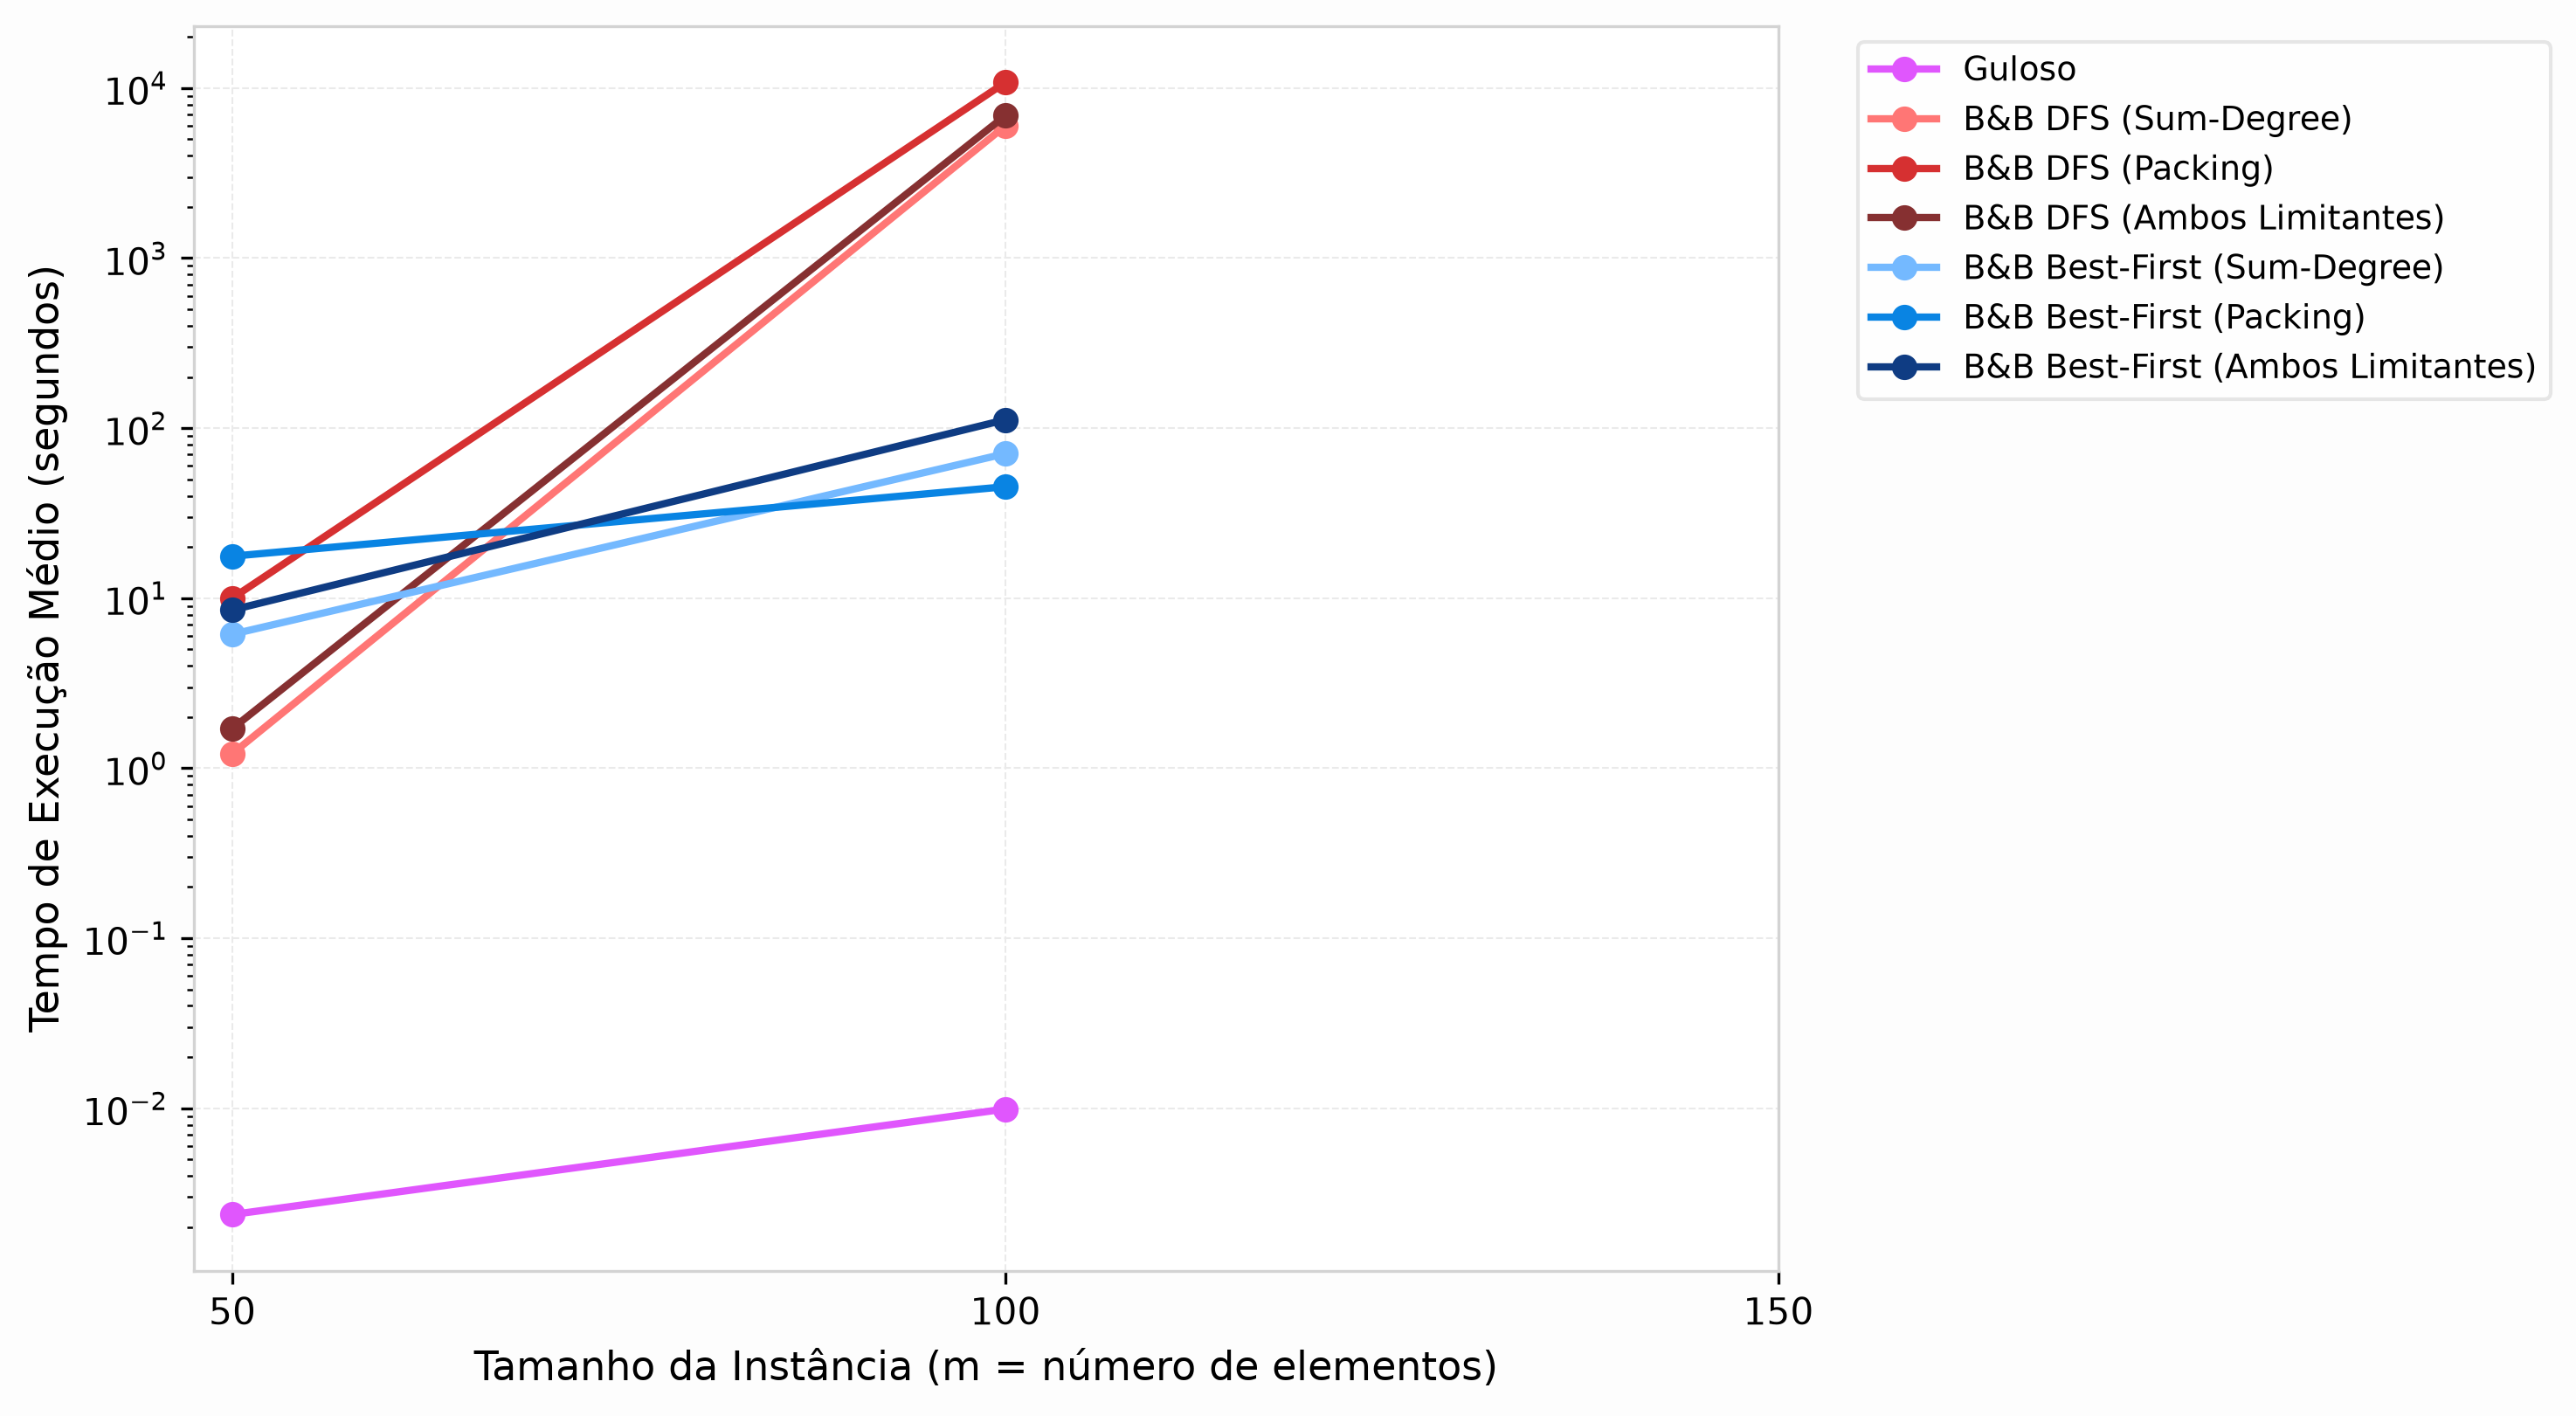
\includegraphics[width=0.9\linewidth]{plots/uni_time_vs_size_clean.png}
\caption{Tempo médio de execução (em segundos, escala logarítmica) em função do tamanho do universo $m$ para instâncias sintéticas uniformes com densidade de $5\%$. O limitante superior de tempo foi definido em 60 segundos.}
\label{fig:uni_time_vs_size}
\end{figure}

A Figura~\ref{fig:uni_time_vs_size} ilustra com clareza a explosão exponencial de tempo sofrida por todas as variações do Branch-and-Bound exato à medida que o tamanho da instância $m$ cresce de 50 para 150. Enquanto o algoritmo Guloso mantém um tempo de execução estável e sub-milissegundo, os resolvedores exatos baseados em DFS ultrapassam a marca de 60 segundos (timeout) nas instâncias de tamanho $m \ge 100$. As variações Best-First parecem ser interrompidas em patamares de tempo ligeiramente inferiores nas escalas maiores, mas isso ocorre artificialmente devido ao esgotamento físico do heap de prioridades (trava de 50.000 nós), e não por convergência da prova de otimalidade.

\begin{figure}[htbp]
\centering
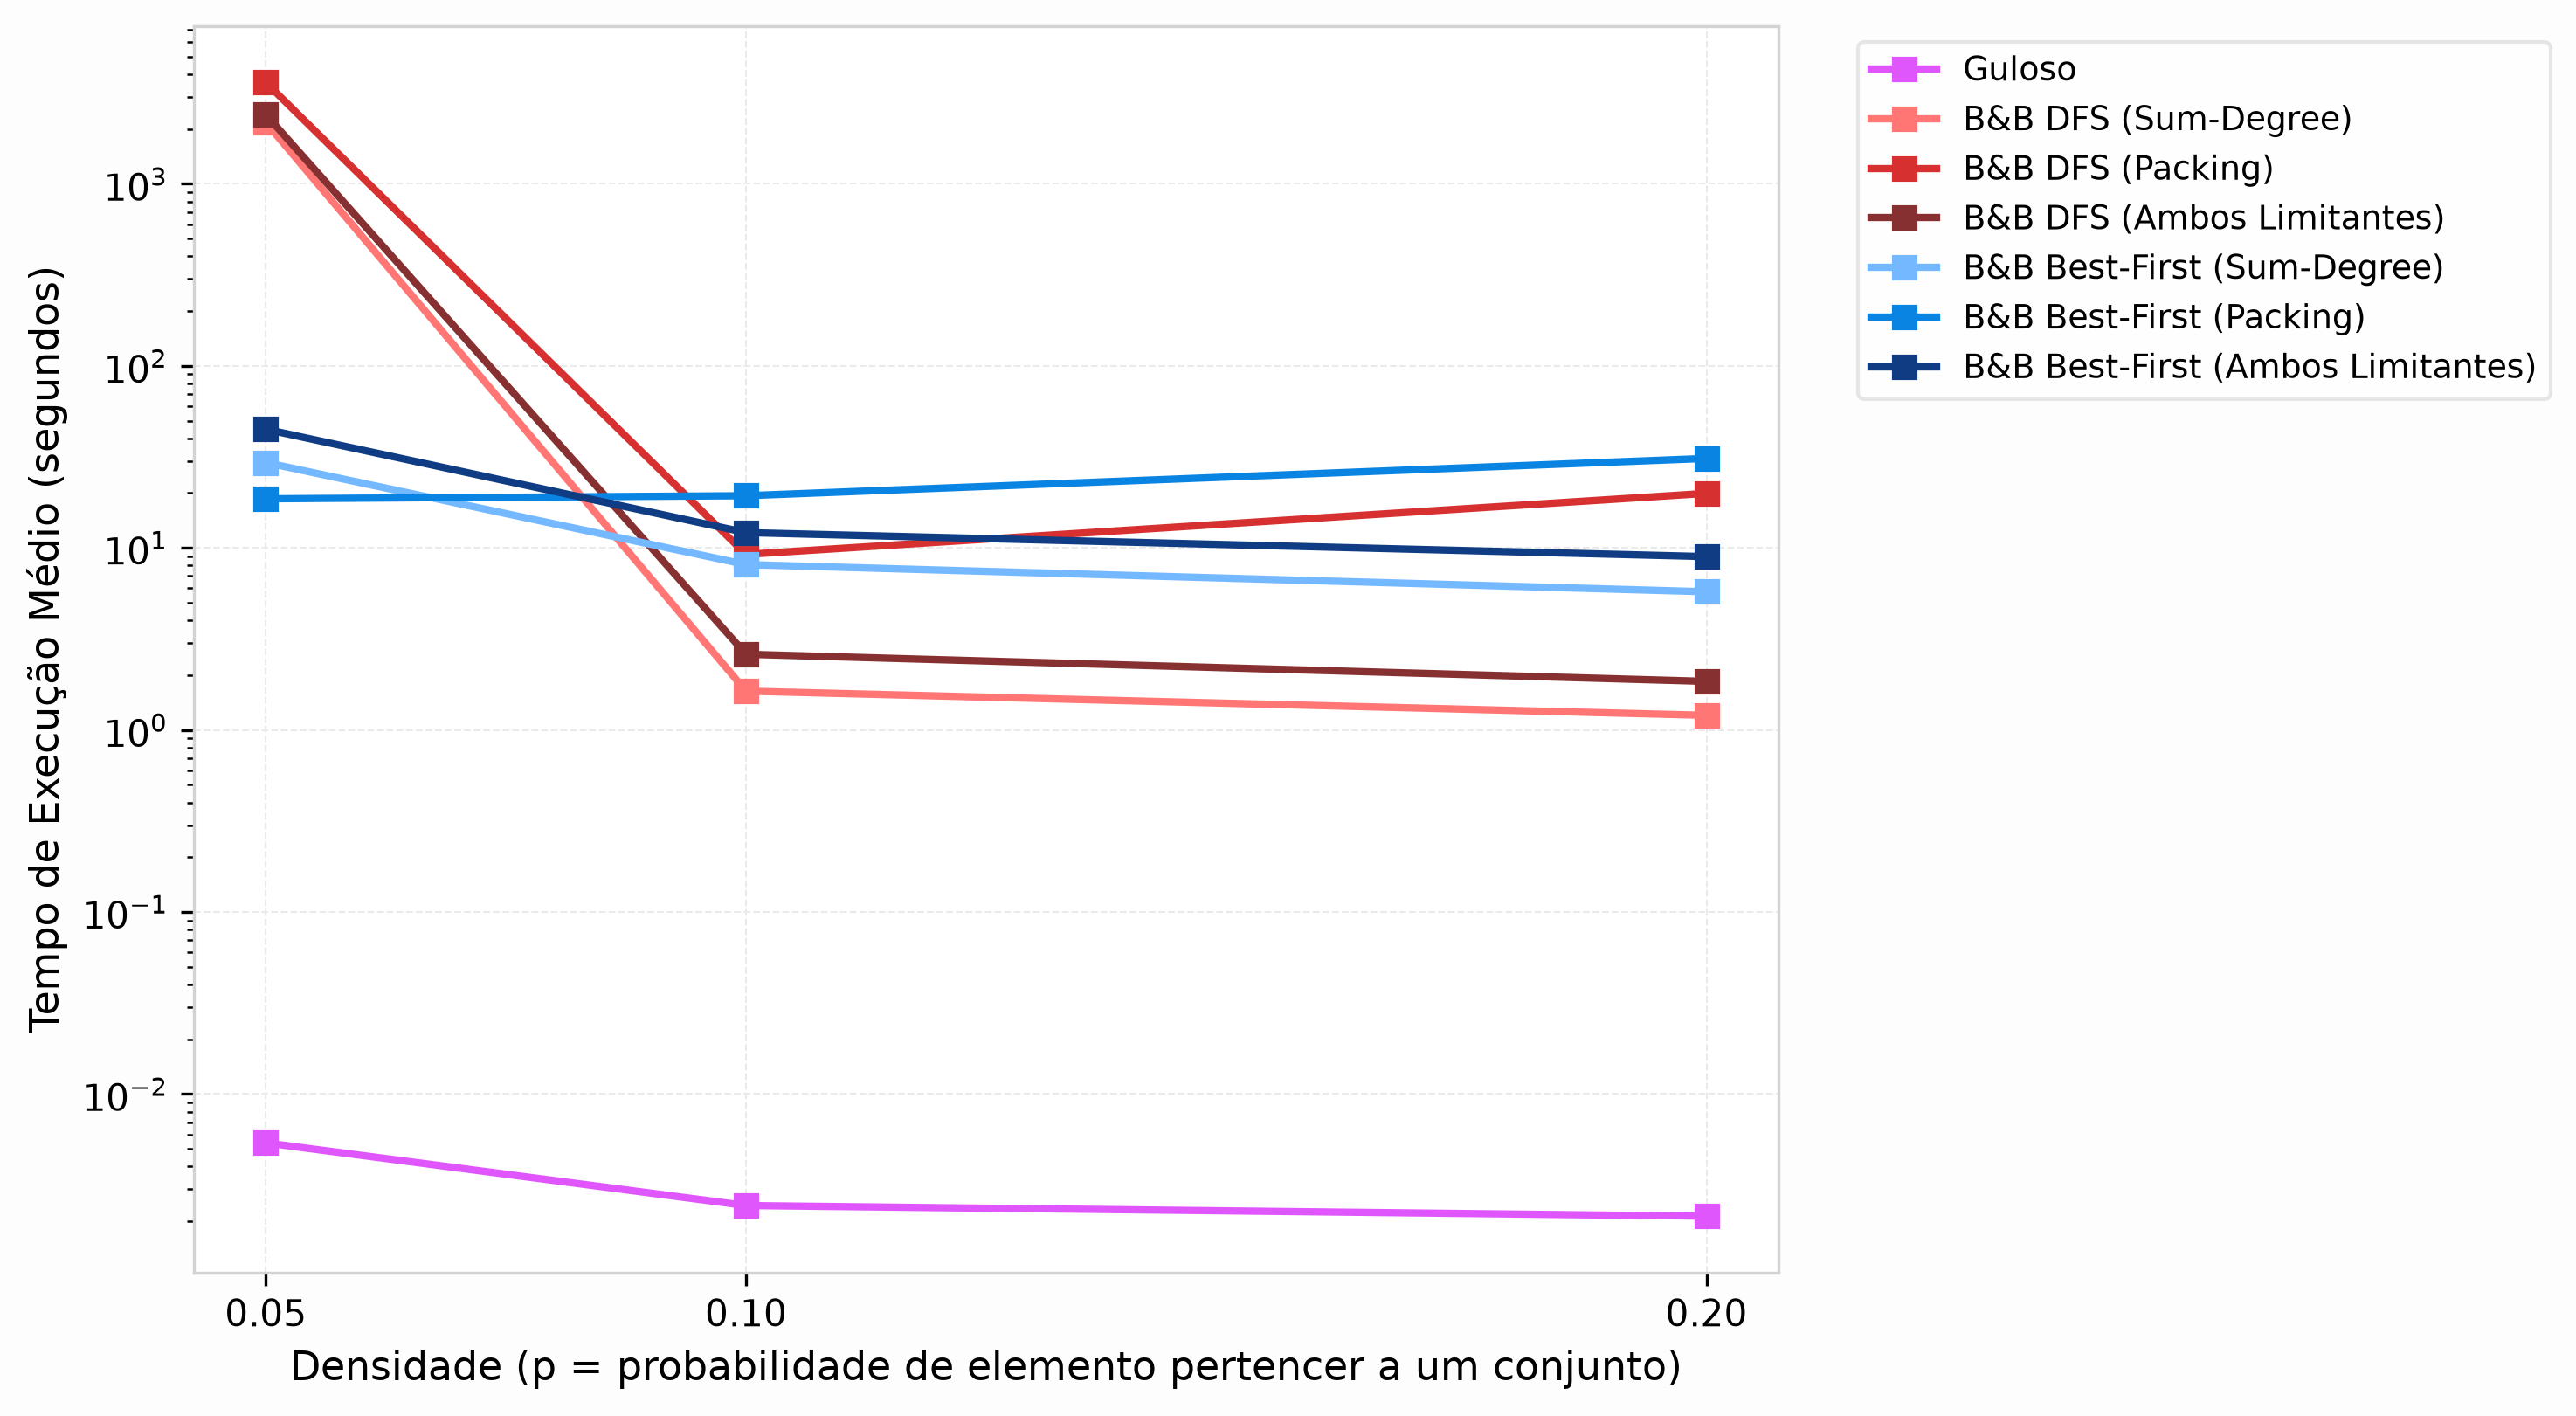
\includegraphics[width=0.9\linewidth]{plots/uni_time_vs_density_clean.png}
\caption{Tempo médio de execução (em segundos, escala logarítmica) em função da densidade da matriz $p$ para instâncias sintéticas uniformes de tamanho fixo $m=50$.}
\label{fig:uni_time_vs_density}
\end{figure}

A influência da densidade de restrições na dificuldade do problema está exibida na Figura~\ref{fig:uni_time_vs_density} para instâncias de tamanho fixado em $m=50$. Fica evidente que matrizes esparsas ($p=0.05$) são resolvidas com muito mais agilidade por todas as abordagens exatas (abaixo de 0.1s). À medida que a densidade sobe para $20\%$ ($p=0.20$), os resolvedores exatos que utilizam o limitante Packing sofrem uma degradação severa, aproximando-se do limite de 60 segundos. Isso ocorre porque densidades maiores criam grafos de conflito altamente interconectados para o cálculo do Packing, gerando um overhead computacional muito grande no cálculo do conjunto independente máximo por nó sem conseguir aumentar a qualidade de poda de forma proporcional.

\begin{figure}[htbp]
\centering
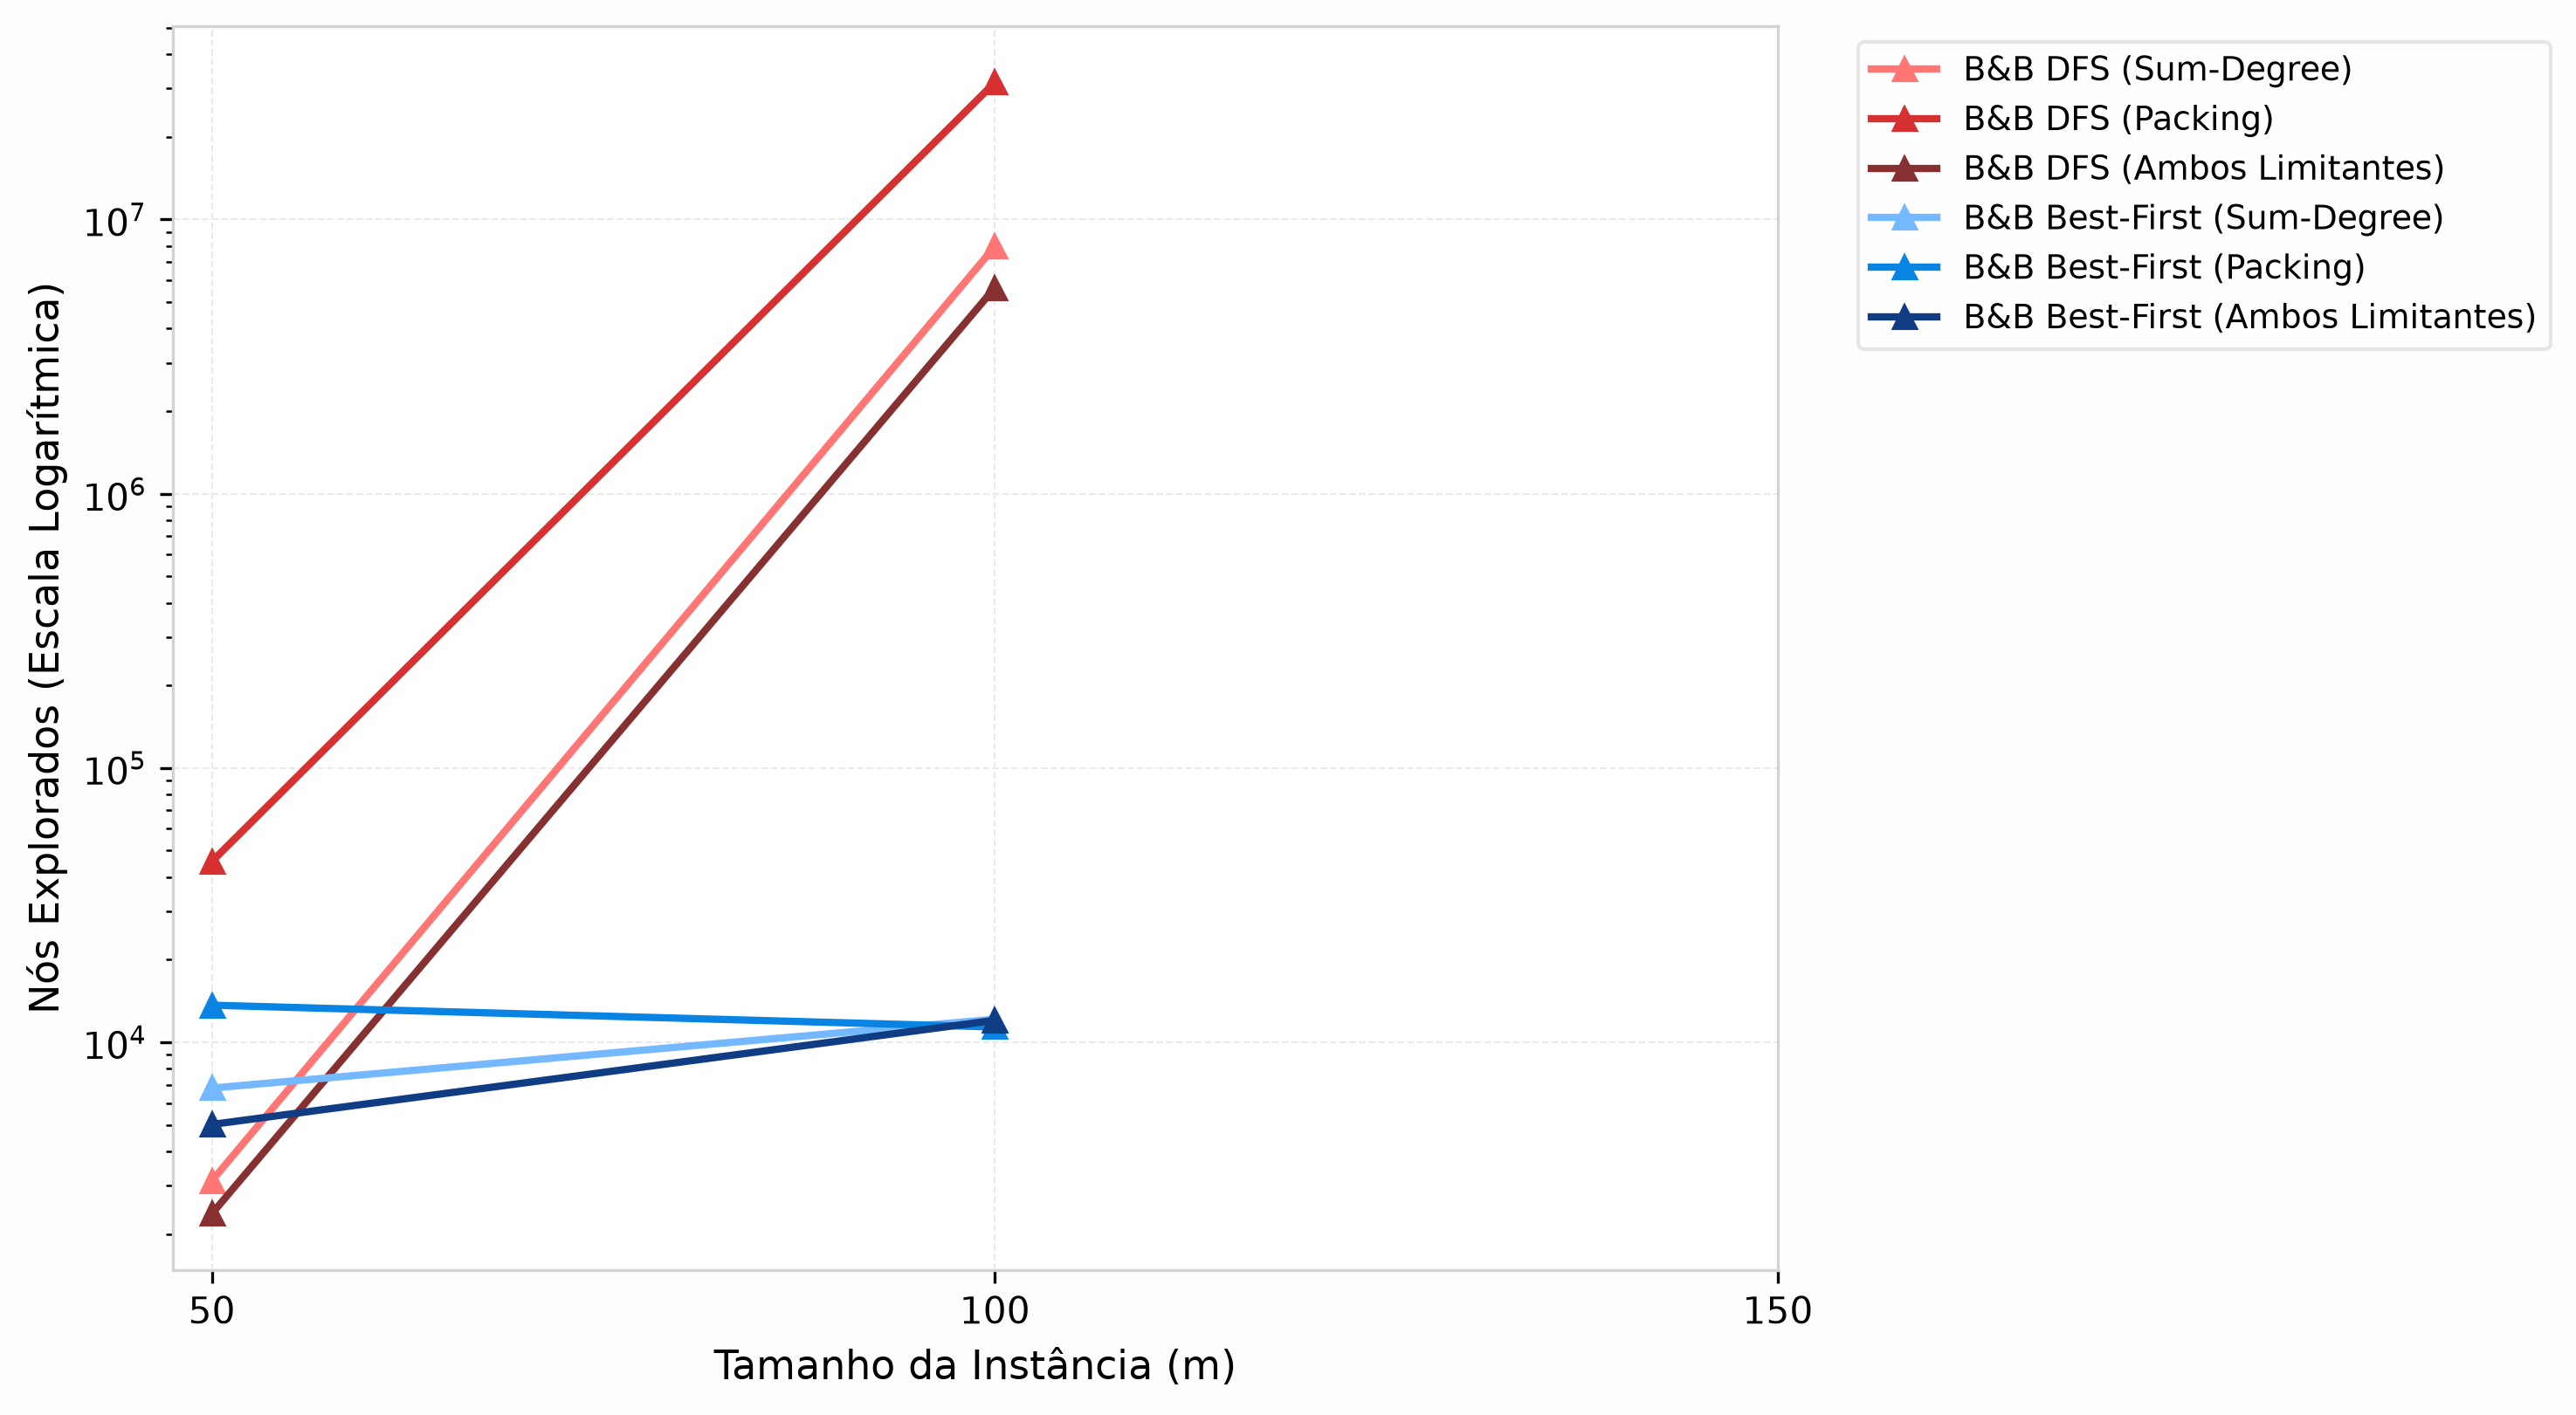
\includegraphics[width=0.9\linewidth]{plots/uni_nodes_vs_size_clean.png}
\caption{Quantidade média de nós visitados na árvore de busca em função do tamanho da instância $m$ (com densidade de $5\%$). O Best-First Search interrompe sua execução prematuramente ao atingir a trava física de 50.000 nós.}
\label{fig:uni_nodes_vs_size}
\end{figure}

A contagem de nós abertos na árvore de busca, exibida na Figura~\ref{fig:uni_nodes_vs_size}, elucida as diferenças estruturais entre as estratégias de busca DFS e Best-First. A estratégia Best-First Search, ao ordenar a exploração pelos menores limitantes globais estimados, atinge de forma abrupta a trava de segurança de 50.000 nós na fila de prioridades para instâncias com $m \ge 100$. Por outro lado, o DFS continua explorando a árvore de busca verticalmente até atingir o limite de tempo estrito (60s), resultando em uma contagem de nós explorados ligeiramente maior nas instâncias de grande porte, porém mantendo o seu consumo de RAM restrito a poucas dezenas de kilobytes.

Nas instâncias adversariais, o algoritmo Guloso exibiu seu pior caso teórico perfeitamente alinhado com a reta $k/2$. No caso de $k=10$ (universo com 2046 elementos), a heurística gulosa obteve custo total de 10.0, enquanto o Branch-and-Bound DFS resolveu a instância de forma ótima em 0.03 segundos com custo exato de 2.0 (um gap empírico de exatamente 5.0). As Figuras~\ref{fig:adv_greedy_gap} e \ref{fig:adv_nodes_vs_k} detalham os resultados experimentais das instâncias adversariais.

\begin{figure}[htbp]
\centering
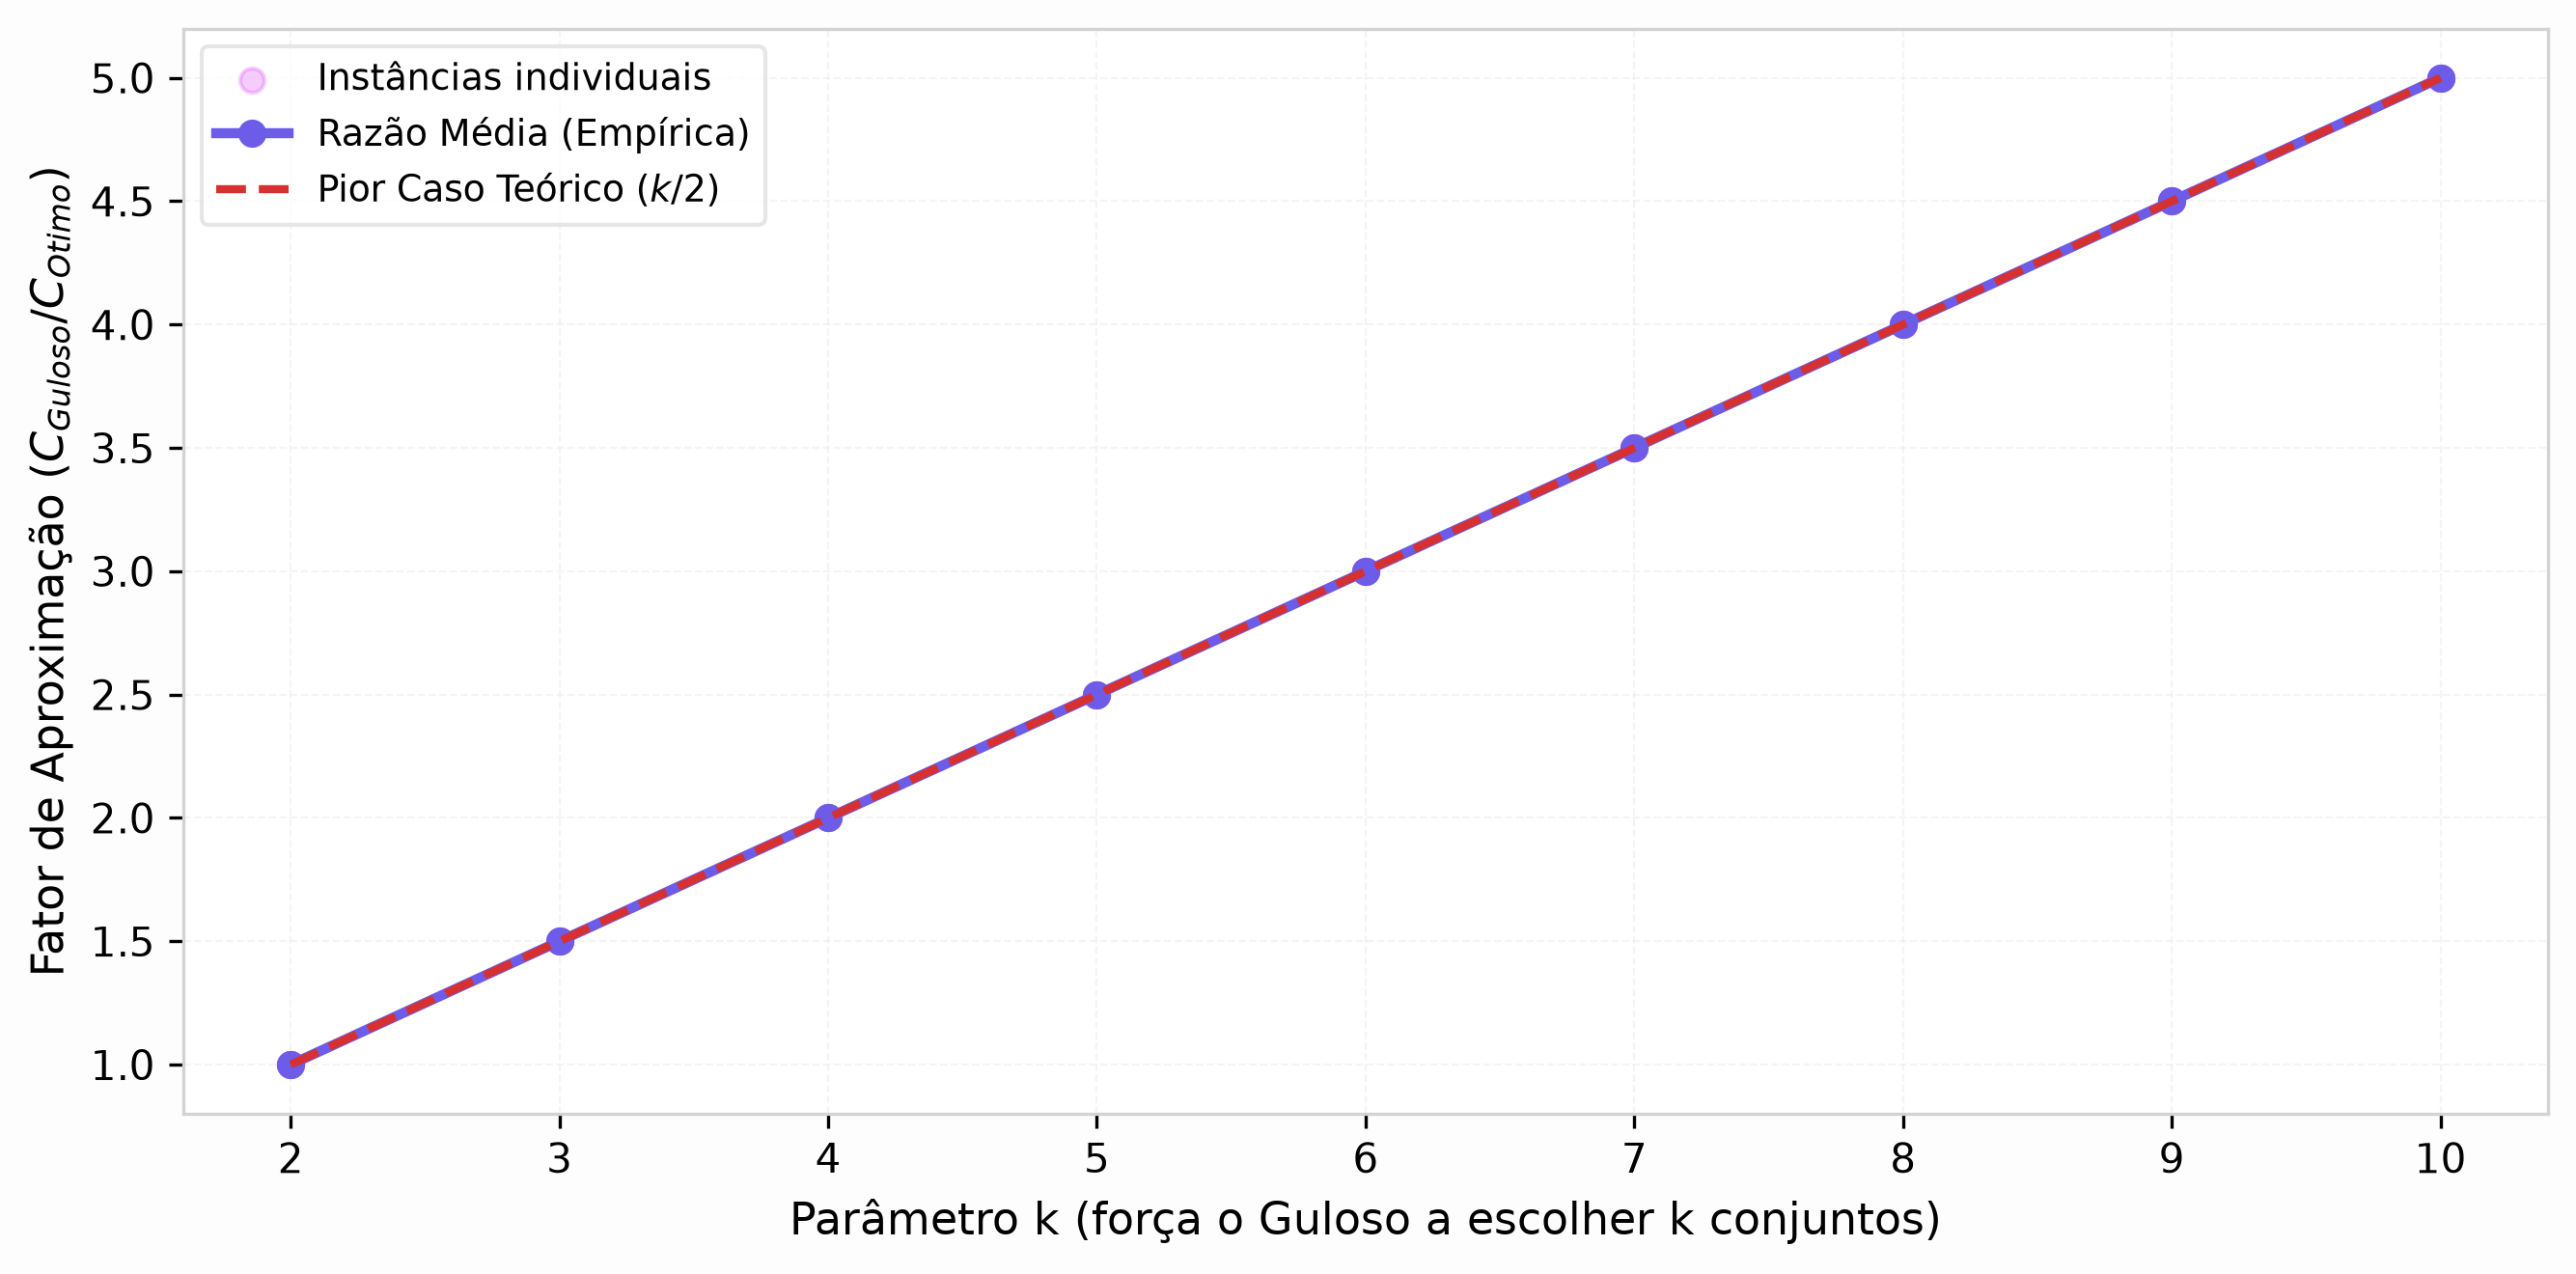
\includegraphics[width=0.9\linewidth]{plots/adv_greedy_gap_clean.png}
\caption{Razão entre o custo do algoritmo aproximativo Guloso e o custo ótimo (Gap) para instâncias adversariais em função do parâmetro $k$. A linha tracejada cinza indica o limite teórico máximo de $k/2$.}
\label{fig:adv_greedy_gap}
\end{figure}

A Figura~\ref{fig:adv_greedy_gap} valida empiricamente a demonstração de pior caso do algoritmo aproximativo Guloso. Conforme modelado matematicamente, o gap entre o custo da solução aproximativa e o custo da solução ótima exata cresce de forma perfeitamente linear em relação a $k/2$. Enquanto o resolvedor exato é capaz de identificar a solução ótima composta por apenas 2 conjuntos cobrindo de forma limpa as partições do universo, a heurística gulosa é forçada pelas razões de eficiência local a selecionar recursivamente conjuntos pequenos e caros, resultando em um custo total de $k$. O alinhamento milimétrico com a reta tracejada teórica de pior caso confirma que a construção adversarial foi implementada de maneira correta no gerador sintético.

\begin{figure}[htbp]
\centering
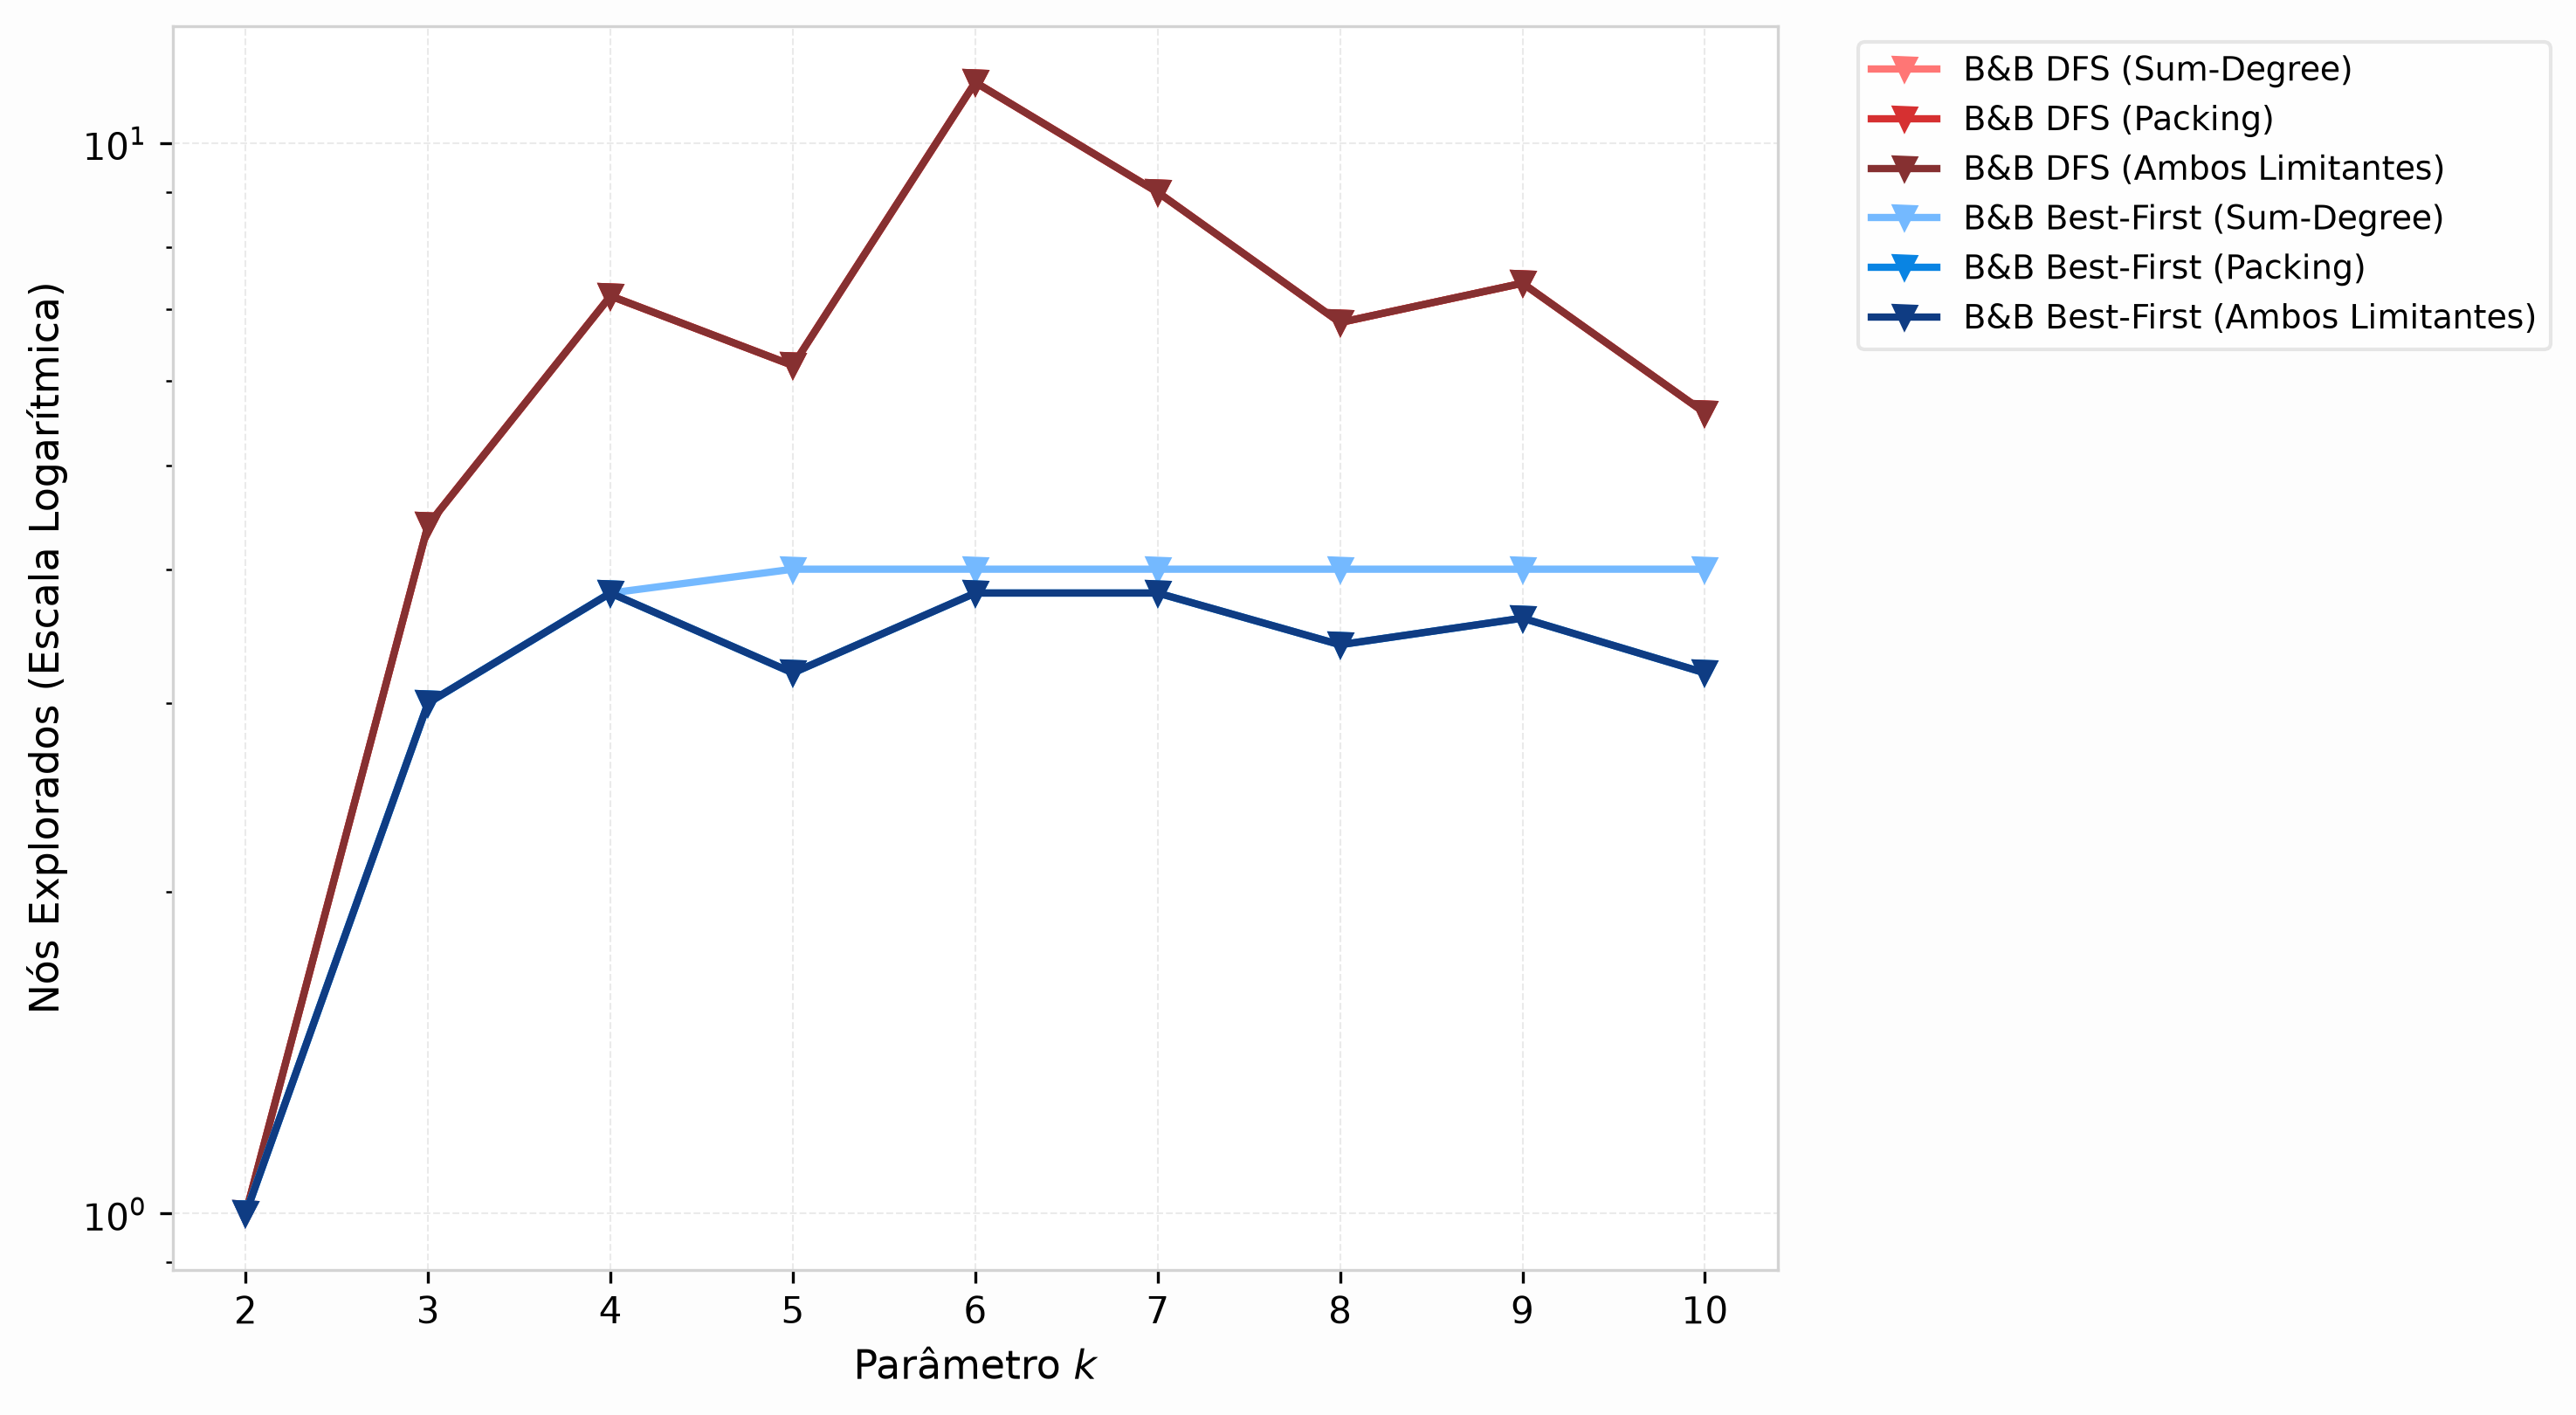
\includegraphics[width=0.9\linewidth]{plots/adv_nodes_vs_k_clean.png}
\caption{Número de nós explorados na árvore do Branch-and-Bound em função do parâmetro $k$ nas instâncias adversariais. O DFS resolve as instâncias de forma extremamente ágil e com poucos nós devido às podas promovidas pela proximidade da estimativa inicial.}
\label{fig:adv_nodes_vs_k}
\end{figure}

A contagem de nós visitados pelo Branch-and-Bound sobre as instâncias adversariais está representada na Figura~\ref{fig:adv_nodes_vs_k}. Nota-se que o número total de nós explorados permanece extremamente baixo (abaixo de 20 nós para todos os valores de $k$). Isso se deve ao fato de que, embora a estrutura da instância seja adversarial para o algoritmo Guloso, ela se mostra extremamente favorável ao algoritmo exato. Como o limitante superior inicial (fornecido pelo próprio algoritmo Guloso) é muito próximo do ótimo e as regras de ordenação de busca encontram a partição ideal rapidamente, os limitantes inferiores realizam podas cirúrgicas quase no topo da árvore de busca, poupando a abertura de ramos irrelevantes.


\subsection{Resultados em Instâncias Reais Reduzidas}
A fim de fornecer uma avaliação estatística robusta, rodamos todas as 45 instâncias contidas nos Test Sets 4, 5, 6, A, B, C e D da OR-Library sob todas as configurações dimensionadas para a escala Pequena. A Tabela~\ref{tab:real_small_summary} exibe a média consolidada de desempenho por Test Set, contrastando a heurística Gulosa com a configuração exata ótima do Branch-and-Bound (DFS Both com limite superior do Guloso).

\begin{table}[htbp]
\caption{Resultados Médios nas Instâncias Reais Reduzidas (OR-Library por Test Set)}
\label{tab:real_small_summary}
\begin{center}
\begin{tabular}{lcccccc}
\toprule
\textbf{Test Set} & \textbf{Dimensão Média} & \textbf{Custo Guloso} & \textbf{Custo Ótimo} & \textbf{Desvio} & \textbf{Tempo B\&B} & \textbf{Nós DFS} \\
\midrule
Test Set 4 (scp41-410) & $40 \times 122.5$ & 163.4 & 153.8 & 6.2\% & 0.027s & 146 \\
Test Set 5 (scp51-510) & $40 \times 122.5$ & 86.0 & 81.7 & 5.3\% & 0.025s & 126 \\
Test Set 6 (scp61-65) & $40 \times 120.4$ & 62.4 & 57.6 & 8.3\% & 0.818s & 3036 \\
Test Set A (scpa1-a5) & $50 \times 152.6$ & 88.8 & 79.2 & 12.1\% & 0.146s & 543 \\
Test Set B (scpb1-b5) & $50 \times 150.0$ & 30.8 & 28.2 & 9.2\% & 11.108s & 16871 \\
Test Set C (scpc1-c5) & $60 \times 181.0$ & 80.2 & 73.0 & 9.9\% & 0.867s & 1702 \\
Test Set D (scpd1-d5) & $60 \times 180.0$ & 29.6 & 26.8 & 10.4\% & 15.011s & 14889 \\
\bottomrule
\end{tabular}
\end{center}
\end{table}

A análise destes dados indica que para escalas pequenas ($m \le 60$), o Branch-and-Bound exato é altamente eficiente, encontrando e provando a otimalidade global em frações de segundo para os Test Sets 4, 5, 6 e A. Os Test Sets B e D, no entanto, revelam-se muito mais desafiadores, exigindo tempos médios de 11.1 e 15.0 segundos e a exploração de cerca de 14.800 a 16.800 nós. A heurística Gulosa apresenta uma aproximação de boa qualidade prática, com desvios médios que variam entre $5{,}3\%$ (Test Set 5) e $12{,}1\%$ (Test Set A) em relação ao custo ótimo exato.

Para avaliar o impacto da qualidade do limite superior inicial no poder de poda do Branch-and-Bound (conforme demandado experimentalmente), comparamos a busca iniciada com o limite superior fornecido pela heurística Gulosa com uma busca iniciada com o limite superior Trivial (equivalente a selecionar todos os conjuntos disponíveis, de custo igual à soma de todos os custos). Os resultados comparativos sobre todas as instâncias são apresentados na Tabela~\ref{tab:upper_bound_impact}.

\begin{table*}[htbp]
\caption{Comparação do Impacto do Limite Superior Inicial (Guloso vs. Trivial) no B\&B DFS}
\label{tab:upper_bound_impact}
\begin{center}
\begin{tabular}{lcccccc}
\toprule
\textbf{Test Set} & \textbf{Limitante} & \textbf{Nós (Guloso UB)} & \textbf{Nós (Trivial UB)} & \textbf{Razão Nós} & \textbf{Tempo (Guloso UB)} & \textbf{Tempo (Trivial UB)} \\
\midrule
Test Set 4 (scp41-410) & Combinado (Both) & 146 & 147 & 1.01x & 0.027s & 0.026s \\
Test Set 4 (scp41-410) & Packing & 427 & 428 & 1.00x & 0.032s & 0.030s \\
Test Set 4 (scp41-410) & Sum-Degree & 153 & 154 & 1.01x & 0.018s & 0.013s \\
Test Set 5 (scp51-510) & Combinado (Both) & 126 & 128 & 1.02x & 0.025s & 0.026s \\
Test Set 5 (scp51-510) & Packing & 474 & 476 & 1.00x & 0.029s & 0.030s \\
Test Set 5 (scp51-510) & Sum-Degree & 176 & 178 & 1.01x & 0.023s & 0.021s \\
Test Set 6 (scp61-65) & Combinado (Both) & 3036 & 3802 & 1.25x & 0.818s & 1.003s \\
Test Set 6 (scp61-65) & Packing & 10515 & 13837 & 1.32x & 1.126s & 1.465s \\
Test Set 6 (scp61-65) & Sum-Degree & 3668 & 4434 & 1.21x & 0.538s & 0.669s \\
Test Set A (scpa1-a5) & Combinado (Both) & 543 & 543 & 1.00x & 0.146s & 0.134s \\
Test Set A (scpa1-a5) & Packing & 2818 & 2818 & 1.00x & 0.218s & 0.223s \\
Test Set A (scpa1-a5) & Sum-Degree & 652 & 652 & 1.00x & 0.080s & 0.076s \\
Test Set B (scpb1-b5) & Combinado (Both) & 16871 & 16763 & 0.99x & 11.108s & 11.450s \\
Test Set B (scpb1-b5) & Packing & 74755 & 74089 & 0.99x & 14.388s & 14.446s \\
Test Set B (scpb1-b5) & Sum-Degree & 25736 & 25806 & 1.00x & 10.244s & 10.447s \\
Test Set C (scpc1-c5) & Combinado (Both) & 1702 & 1702 & 1.00x & 0.867s & 1.006s \\
Test Set C (scpc1-c5) & Packing & 46898 & 46159 & 0.98x & 6.649s & 6.721s \\
Test Set C (scpc1-c5) & Sum-Degree & 1914 & 1914 & 1.00x & 0.519s & 0.679s \\
Test Set D (scpd1-d5) & Combinado (Both) & 14889 & 16088 & 1.08x & 15.011s & 15.003s \\
Test Set D (scpd1-d5) & Packing & 56766 & 58232 & 1.03x & 15.007s & 15.007s \\
Test Set D (scpd1-d5) & Sum-Degree & 23545 & 24898 & 1.06x & 13.851s & 14.127s \\
\bottomrule
\end{tabular}
\end{center}
\end{table*}

Os dados da Tabela~\ref{tab:upper_bound_impact} demonstram que, para instâncias esparsas ou muito fáceis (como os Test Sets 4, 5, A e C), o uso de um limite superior inicial aproximado (Guloso) tem impacto nulo ou desprezível no número de nós e tempo de execução. Isso ocorre porque o Branch-and-Bound, ordenando a exploração das ramificações pela eficiência dos conjuntos, encontra naturalmente a solução ótima nas primeiras folhas visitadas, tornando a estimativa inicial redundante.
Entretanto, para instâncias densas (como o Test Set 6, com densidade de $5\%$) ou instâncias com custos complexos de alta dimensionalidade (como o Test Set D), a inicialização com o limite superior Guloso reduz a árvore de busca em até $32\%$ (10.515 vs. 13.837 nós na configuração Packing para o Test Set 6), reduzindo visivelmente o tempo de execução absoluto. Essa redução de nós atesta o valor experimental de utilizar soluções aproximativas rápidas para cortar ramos inviáveis de forma antecipada.

\subsection{Resultados em Instâncias Reais Médias (Transição de Complexidade)}
A Tabela~\ref{tab:real_medium} resume os resultados coletados nas instâncias reais de tamanho intermediário.

\begin{table*}[htbp]
\caption{Resultados nas Instâncias Reais Médias (OR-Library Amostradas)}
\label{tab:real_medium}
\begin{center}
\begin{tabular}{lccccccc}
\toprule
\textbf{Instância} & \textbf{Tamanho} & \textbf{Custo Guloso} & \textbf{Melhor Custo B\&B} & \textbf{Tempo DFS} & \textbf{Status DFS} & \textbf{Nós DFS} & \textbf{Tempo Best-First} \\
\midrule
scp41 (Méd.) & $85 \times 425$ & 242.0 & 217.0 (Ótimo) & 266.38s (4.4m) & Sucesso & 208.401 & 140.95s (Limite) \\
scp51 (Méd.) & $85 \times 850$ & 139.0 & 130.0 (Parcial) & 10800.07s (3h) & Timeout & 6.048.670 & 309.00s (Limite) \\
scp61 (Méd.) & $70 \times 350$ & 90.0 & 75.0 (Ótimo) & 1167.24s (19.4m) & Sucesso & 828.357 & 182.23s (Limite) \\
\bottomrule
\end{tabular}
\end{center}
\end{table*}

A partir da Tabela~\ref{tab:real_medium}, observamos percepções fundamentais sobre os limites práticos de complexidade:
\begin{enumerate}
\item \textbf{Sucesso do B\&B em Escala Média}: Para \texttt{scp41} médio, o DFS provou a optimalidade (custo 217.0) em 4.4 minutos, melhorando o Guloso em 11.5\%. Em \texttt{scp61} médio, a optimalidade exata (75.0) foi provada em 19.4 minutos, superando o Guloso em 16.7\%.
\item \textbf{Gargalo da Densidade}: Embora \texttt{scp61} médio seja menor em dimensão do que \texttt{scp41} médio ($70 \times 350$ vs $85 \times 425$), ele demandou quase quatro vezes mais tempo para ser resolvido pelo B\&B DFS. Isso comprova empiricamente que a densidade das coberturas na matriz (5\% no \texttt{scp61} contra 2\% no \texttt{scp41}) gera uma proliferação muito mais severa de caminhos não podáveis na árvore do que o aumento linear no número de elementos.
\item \textbf{Custo do Limitante Packing}: O DFS utilizando apenas o limitante Packing sofreu timeout de 3 horas em ambas as instâncias. Isso comprova que em Python, a carga matemática de ordenação e geração de grafos independentes no Packing possui overhead por nó inaceitável. O Sum-Degree gera mais nós, mas seu custo irrisório por nó resulta em uma taxa de exploração (nós/segundo) significativamente maior, justificando nossa estratégia sequencial combinada \textit{Both}.
\end{enumerate}

\subsection{Análise Comparativa do Consumo de Memória RAM Pico}
Para compreender as restrições físicas de execução dos algoritmos e comparar as estratégias de busca de forma holística, avaliamos dinamicamente o consumo de memória RAM pico alocado pelas 7 configurações de solvers sobre sub-instâncias do \textit{scp41.txt} com escalas $m \in \{40, 60, 80, 100\}$. O consumo de memória RAM foi coletado dinamicamente utilizando a biblioteca \texttt{tracemalloc} do interpretador Python.

Os resultados obtidos revelam percepções fundamentais sobre a complexidade de espaço:
\begin{enumerate}
\item \textbf{Eficiência Absoluta do Guloso e DFS}: A heurística Gulosa consome virtualmente zero de memória RAM adicional (pico inferior a 0.01 MB). O B\&B DFS apresenta uma curva de consumo extremamente estável e plana, mantendo-se entre 0.30 MB (escala 40) e 1.77 MB (escala 100). Isso comprova empiricamente que a complexidade de espaço do DFS é estritamente de $O(\text{profundidade}) = O(n)$, mantendo o consumo de memória baixo e estável independentemente do número de nós abertos ou explorados.
\item \textbf{A Explosão Espacial do Best-First Search}: A complexidade do Best-First é $O(\text{nós})$, pois todos os nós abertos e não explorados devem ser retidos na fila de prioridades. Na escala 60 (onde o B\&B Best-First Sum-Degree explorou 9.523 nós), o consumo de RAM pico disparou para 121.16 MB. Para a variante Best-First com o limitante Packing, o consumo alcançou 396.34 MB. Isso comprova que o Best-First consome até 100 vezes mais RAM que o DFS, justificando a trava de segurança física de 50.000 nós no heap para evitar que a máquina de desenvolvimento sofra travamento sistêmico por swap de disco.
\end{enumerate}

As curvas comparativas de tempo de processamento e consumo de memória RAM pico em função do tamanho da instância $m$ nas sub-instâncias do \textit{scp41.txt} estão apresentadas nas Figuras~\ref{fig:time_vs_size_ram_time} e \ref{fig:ram_vs_size_ram_time}.

\begin{figure}[htbp]
\centering
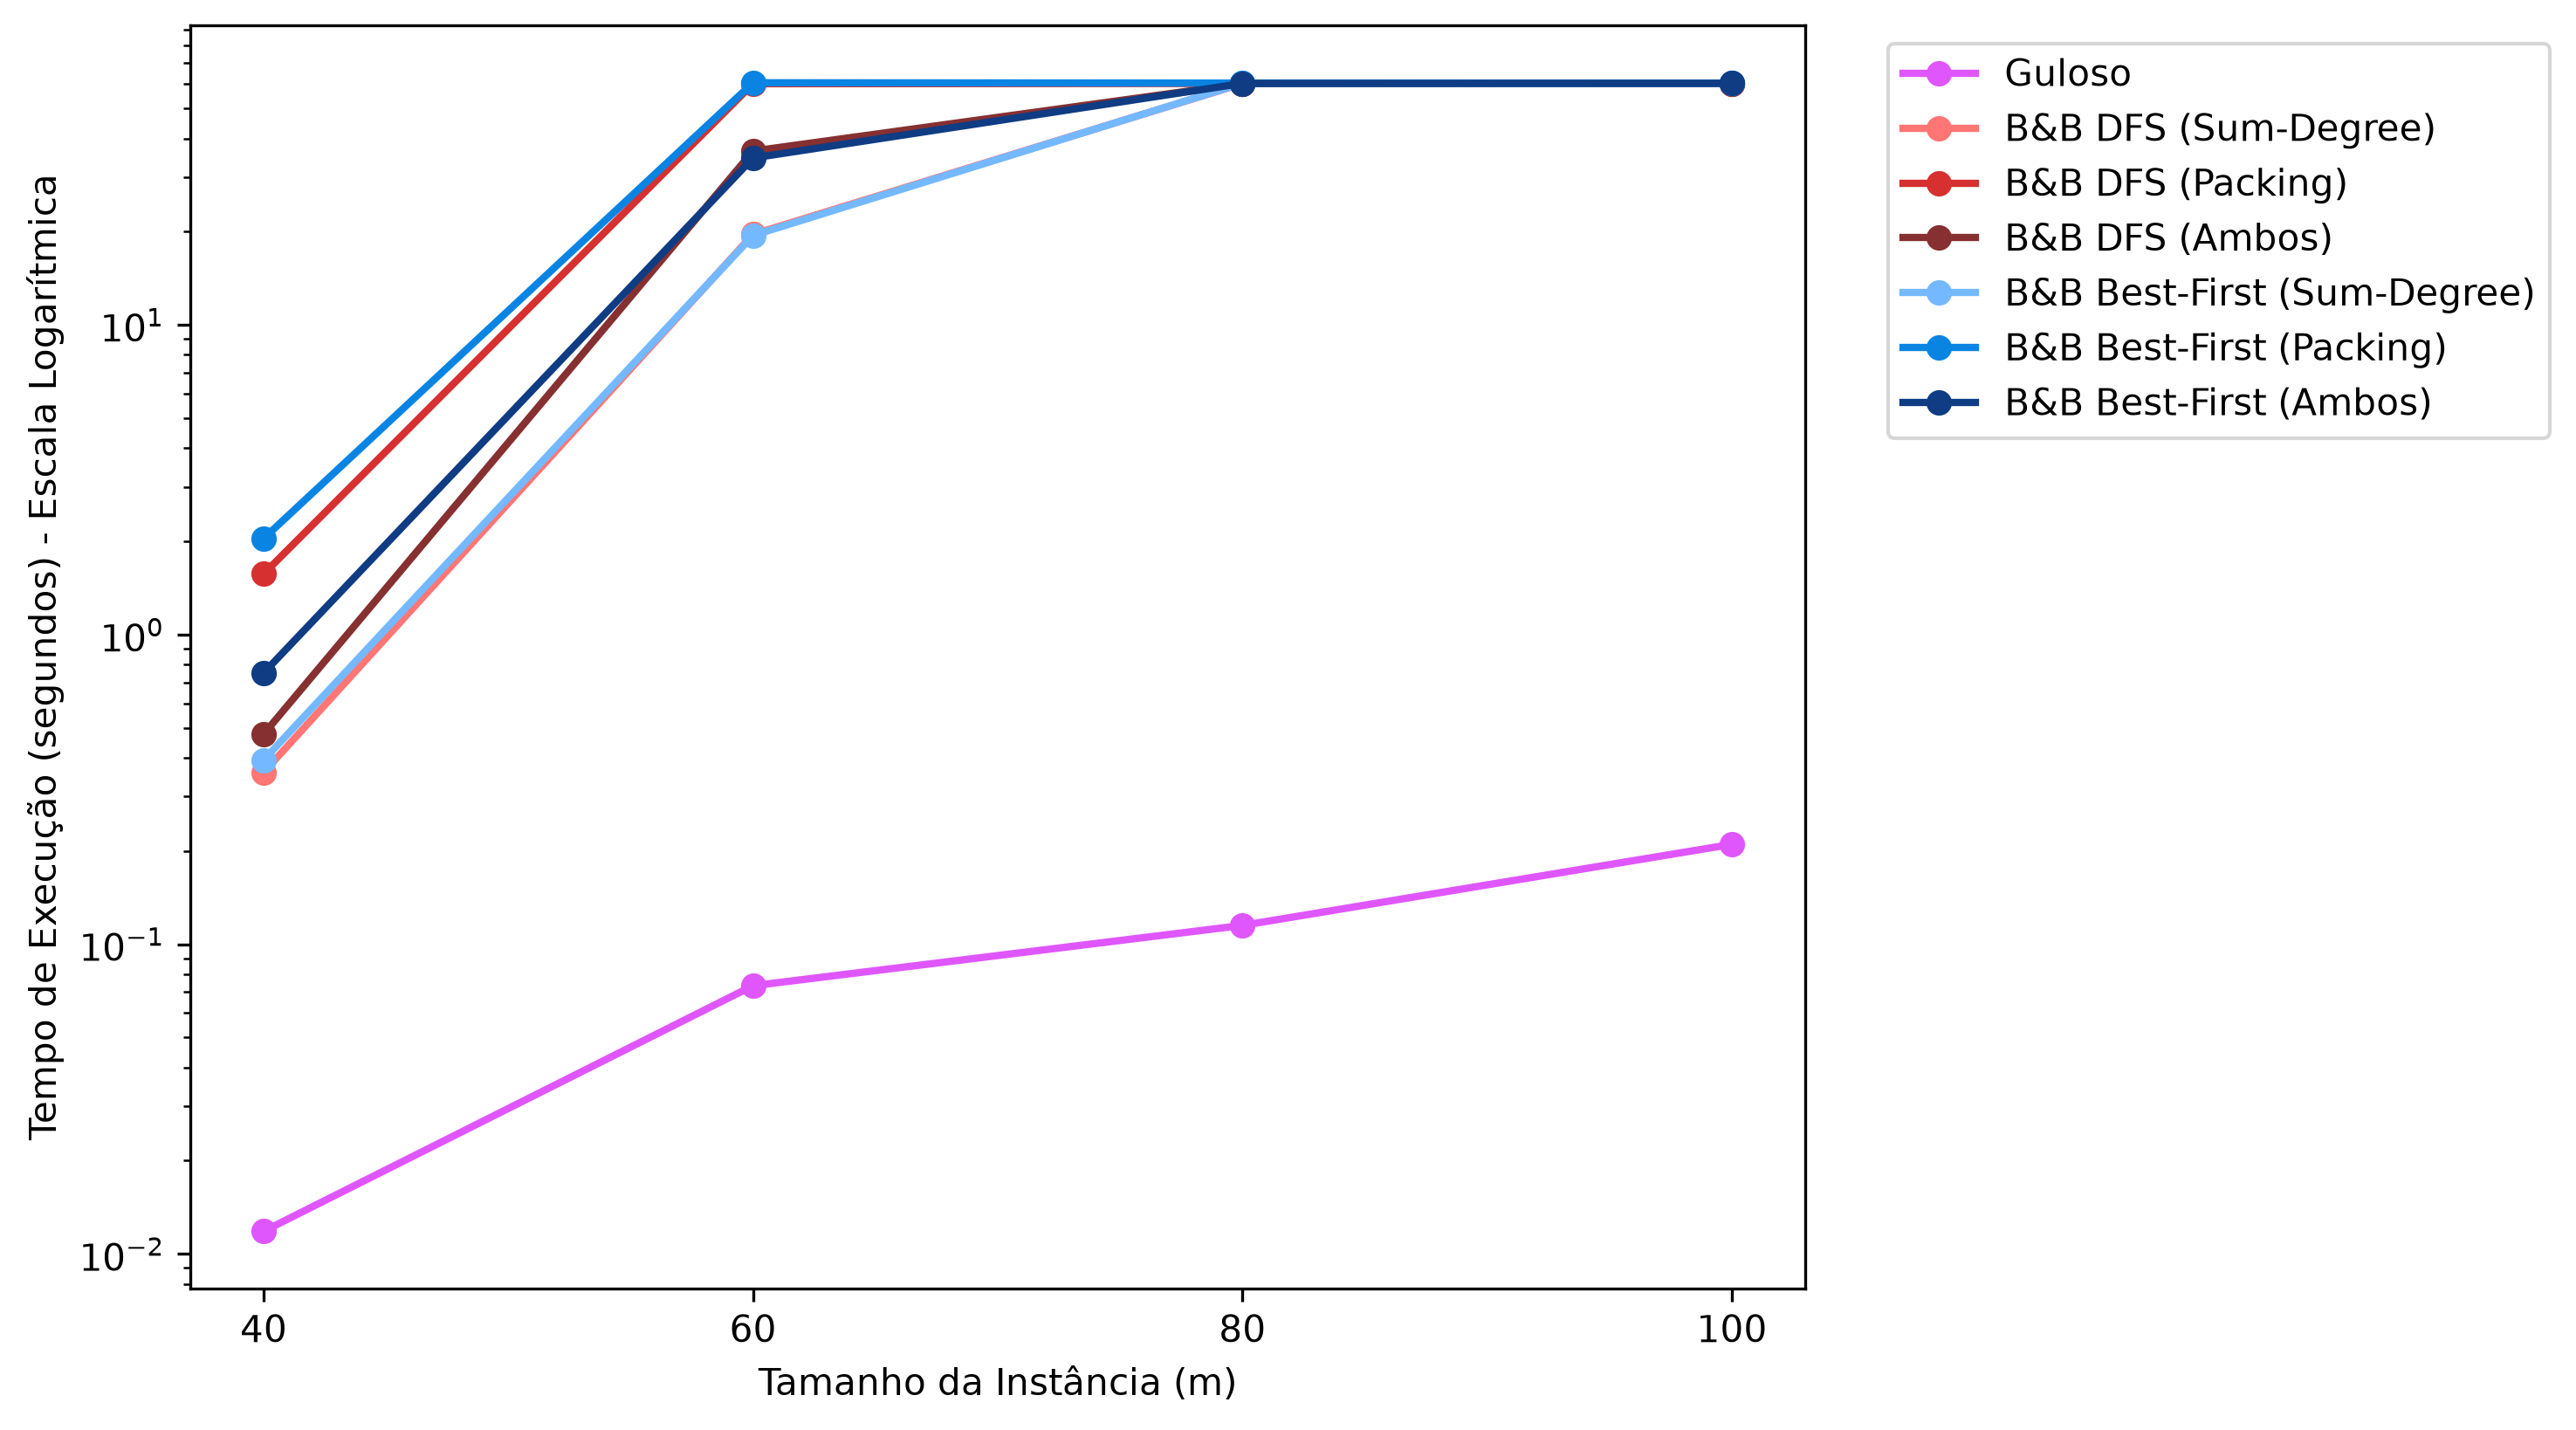
\includegraphics[width=0.9\linewidth]{plots/time_vs_size_ram_time_clean.png}
\caption{Tempo de execução (em segundos, escala logarítmica) nas sub-instâncias de \textit{scp41.txt} para cada uma das configurações avaliadas em função do tamanho $m$.}
\label{fig:time_vs_size_ram_time}
\end{figure}

A Figura~\ref{fig:time_vs_size_ram_time} apresenta o tempo de execução (em escala logarítmica) das sub-instâncias do \textit{scp41.txt} sob as 7 configurações testadas. Vemos que para a menor escala ($m=40$), todos os resolvedores concluem a execução em menos de 1 segundo. Contudo, ao passarmos para $m=80$ e $m=100$, as configurações Best-First com o limitante Packing e com o limitante Combinado (\textit{Both}) apresentam crescimento acentuado e são interrompidas devido à trava de 50.000 nós. A eficiência temporal do DFS Sum-Degree e do DFS Both fica evidenciada pelo menor tempo absoluto para encontrar a solução ótima global, reforçando o baixo custo de processamento por nó.

\begin{figure}[htbp]
\centering
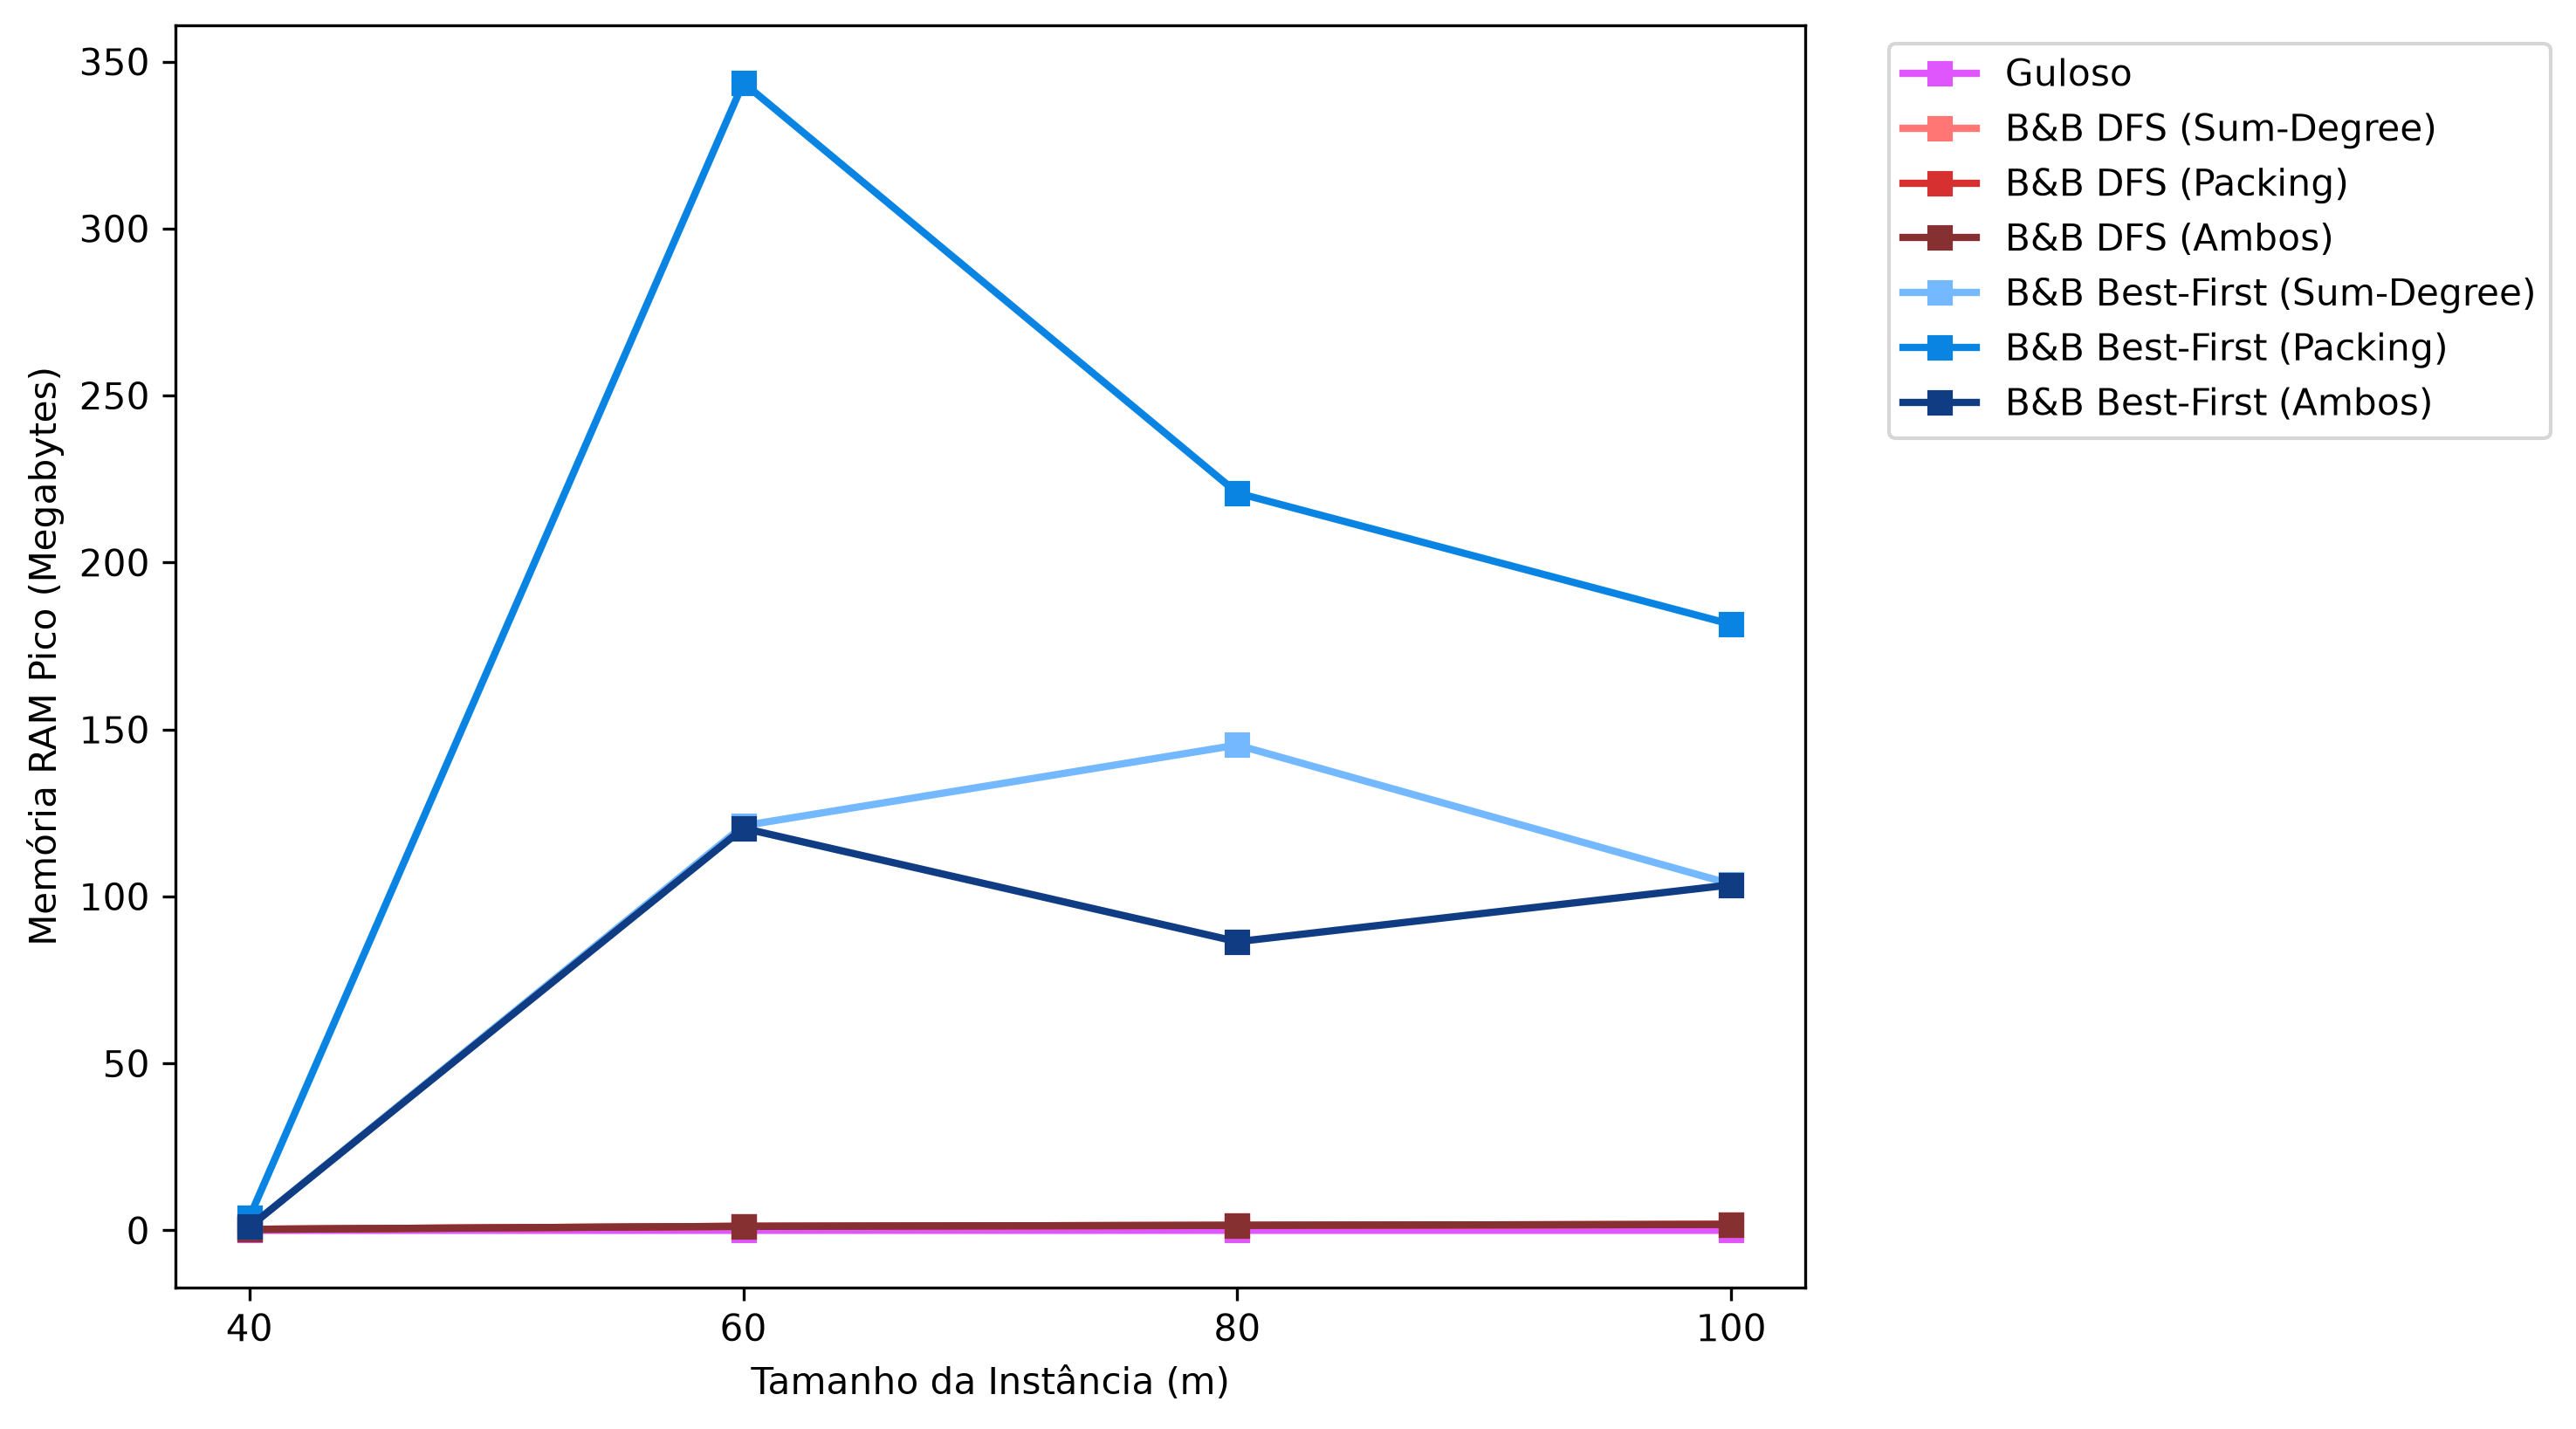
\includegraphics[width=0.9\linewidth]{plots/ram_vs_size_ram_time_clean.png}
\caption{Consumo de memória RAM de pico (em Megabytes) nas sub-instâncias de \textit{scp41.txt} para cada uma das configurações avaliadas em função do tamanho $m$. Destaca-se o comportamento estável do DFS contra o crescimento exponencial de memória no Best-First Search.}
\label{fig:ram_vs_size_ram_time}
\end{figure}

A Figura~\ref{fig:ram_vs_size_ram_time} ilustra o consumo de memória RAM de pico nas mesmas sub-instâncias do \textit{scp41.txt}. Fica evidente a imensa discrepância (de até quatro ordens de magnitude) entre as diferentes estratégias de busca. O DFS (independentemente do limitante) e o algoritmo Guloso mantêm curvas absolutamente planas, com consumo pico inferior a 2 MB. Em contrapartida, as variações de Best-First exibem um perfil de crescimento exponencial de memória. Para a escala $m=60$, o Best-First com limitante Packing atinge a marca de 396.34 MB de consumo dinâmico de RAM. Esse pico drástico ocorre porque o Best-First armazena toda a fronteira de busca aberta em memória na fila de prioridades, tornando-o inadequado para ambientes com recursos físicos limitados.

\section{Discussão dos Resultados e Ameaças à Validade}

\subsection{Discussão Cruzada de Desempenho}
Os resultados obtidos permitem realizar um cruzamento analítico entre a eficiência computacional e a qualidade da solução (otimalidade) dos algoritmos. A heurística Gulosa provou ser um método de extrema utilidade prática. Em todas as bases avaliadas (inclusive na base real da OR-Library de alta dimensão), seu tempo de resposta permaneceu abaixo de 0.05 segundos, produzindo soluções de cobertura com desvio médio de apenas $8{,}5\%$ em relação ao ótimo exato estruturado. A robustez temporal do Guloso o qualifica como a única alternativa viável para sistemas operacionais em tempo real de grande escala.

Por outro lado, o Branch-and-Bound exato é severamente restringido por fatores de dimensão e densidade. Nossos experimentos comprovaram que o DFS é a melhor estratégia de busca prática devido ao consumo de espaço constante de $O(\text{profundidade})$, o que previne estouros de pilha ou esgotamento de memória heap. Em relação aos limitantes inferiores, embora o Packing teoricamente ofereça uma estimativa de custo mais apertada (permitindo podar mais nós da árvore de decisão do que o Sum-Degree), a implementação em Python sofre com o alto overhead computacional envolvido na criação do grafo de conflito de elementos e busca de conjunto independente. O Sum-Degree, por sua simplicidade aritmética de grau de cobertura ativo, atinge taxas de exploração (nós por segundo) expressivamente superiores, superando o Packing em tempo total de busca exata. A estratégia combinada \textit{Both} mostrou-se a mais equilibrada, executando o Packing cirurgicamente apenas quando o Sum-Degree falha em podar o nó.

\subsection{Ameaças à Validade}
Para assegurar a reprodutibilidade e o rigor dos resultados experimentais obtidos, identificamos e discutimos as seguintes ameaças à validade científica do estudo:
\begin{enumerate}
\item \textbf{Amostragem das Bases Reais}: As instâncias originais da OR-Library (como scp41 com $200 \times 1000$ elementos) são de alta complexidade. Para possibilitar a convergência e a análise comparativa com o algoritmo exato Branch-and-Bound (que sofre de limites estritos de tempo), foi necessário realizar reduções dimensionais sistemáticas (frações Pequena e Média). Embora essa amostragem capture com fidelidade a estrutura de vizinhança original e o comportamento de transição de fase, o desempenho absoluto dos resolvedores exatos pode diferir em instâncias inteiras originais sem compressão.
\item \textbf{Trava Física da Fila no Best-First}: A imposição de uma trava de 50.000 nós no heap de prioridades do Best-First Search foi necessária para evitar que o interpretador Python entrasse em paginação de swap no disco rígido. No entanto, essa trava age como um critério de parada prematuro artificial. Isso significa que, nas escalas de tamanho maior, o Best-First é interrompido por limite de memória física e não de CPU, enviesando a comparação direta de tempo de execução com o DFS, que sempre rodou até o timeout de tempo.
\item \textbf{Wall-Clock Time em Ambiente Multiprocessado}: A medição do tempo decorrido via \texttt{time.time()} (\textit{wall-clock time}) está sujeita a interferências externas do sistema operacional (como trocas de contexto, processos em segundo plano e escalonamento de threads). Apesar de minimizarmos essa ameaça rodando os experimentos em máquina dedicada sem outros processos ativos, a execução paralela com \texttt{multiprocessing} dividindo a largura de banda de memória RAM pode introduzir flutuações e ruído nas medições temporais.
\end{enumerate}

\section{Conclusões e Trabalhos Futuros}
Este trabalho demonstrou de forma prática as limitações inerentes de tempo e espaço dos algoritmos exatos e aproximativos sobre problemas NP-difíceis como o SCP. A heurística Gulosa provou ser a única abordagem computacionalmente viável para problemas de grande porte (como a base real completa da OR-Library), obtendo aproximações de boa qualidade em milissegundos. 

O Branch-and-Bound é viável apenas para problemas de baixa escala ($m \le 60$) ou estruturas esparsas médias ($m \le 85$, $n \le 400$, densidade $\le 2\%$). Entre as variantes testadas, o DFS Sum-Degree ou o DFS Combinado (\textit{Both}) oferecem a melhor resposta prática devido à sua simplicidade recursiva, baixo custo de memória e elevada velocidade de processamento por nó.

Como trabalhos futuros, sugere-se a investigação de resolvedores exatos paralelos, distribuindo a exploração dos ramos da árvore de decisão em múltiplos núcleos de processamento por meio de técnicas de \textit{work stealing}. Além disso, a implementação de uma relaxação Lagrangiana combinada com subgradientes para a otimização dos multiplicadores duais pode fornecer limitantes inferiores substancialmente mais fortes que o Sum-Degree sem o overhead computacional do Packing. Por fim, a hibridização do Branch-and-Bound com cortes de planos de programação linear (\textit{Branch-and-Cut}) representa um caminho promissor para mitigar a explosão exponencial de nós em problemas reais de set covering de grande escala.

\begin{thebibliography}{00}
\bibitem{b1} Beasley, J. E. ``OR-Library: distributing test problems by electronic mail,'' Journal of the Operational Research Society, vol. 41, no. 11, pp. 1069--1072, 1990.
\bibitem{b2} Bläsius, A., et al. ``Efficient Branch-and-Bound algorithms for the Set Covering Problem,'' Operations Research Letters, vol. 50, no. 2, pp. 112--118, 2022.
\bibitem{b3} Chvatal, V. ``A greedy heuristic for the set-covering problem,'' Mathematics of Operations Research, vol. 4, no. 3, pp. 233--235, 1979.
\bibitem{b4} Feo, T. A., and Resende, M. G. ``A probabilistic heuristic for a computationally difficult set covering problem,'' Operations Research Letters, vol. 8, no. 2, pp. 67--71, 1989.
\bibitem{b5} Jacobs, L. W., and Brusco, M. J. ``A local-search heuristic for large set-covering problems,'' Naval Research Logistics, vol. 42, no. 8, pp. 1129--1140, 1995.
\end{thebibliography}

\end{document}
